% Created 2017-03-17 Fri 16:30
% Intended LaTeX compiler: pdflatex
\documentclass[10pt, openright, notitlepage]{scrreprt}
\usepackage[utf8]{inputenc}
\usepackage[T1]{fontenc}
\usepackage{graphicx}
\usepackage{grffile}
\usepackage{longtable}
\usepackage{wrapfig}
\usepackage{rotating}
\usepackage[normalem]{ulem}
\usepackage{amsmath}
\usepackage{textcomp}
\usepackage{amssymb}
\usepackage{capt-of}
\usepackage{hyperref}
\usepackage{minted}
\usepackage[a4paper, left=25mm, right=25mm, top=27mm, headheight=20mm, headsep=10mm, textheight=242mm, footskip=15mm]{geometry}
\usepackage[backend=biber, style=ieee, natbib=true, url=false, doi=true, eprint=false]{biblatex}
\usepackage[dvipsnames]{xcolor}
% Definition of colors
%---------------------------------------------------------------------------
\RequirePackage{color}
\definecolor{linkblue}{rgb}{0,0,0.8}       % Standard
\definecolor{darkblue}{rgb}{0,0.08,0.45}   % Dark blue
\definecolor{bfhgrey}{rgb}{0.41,0.49,0.57} % BFH grey
\definecolor{linkcolor}{rgb}{0,0,0}
\colorlet{Black}{black}
\definecolor{keywords}{rgb}{255,0,0}
\definecolor{red}{rgb}{0.6,0,0}
\definecolor{green}{rgb}{0,0.5,0}
\definecolor{blue}{rgb}{0,0,0.5}
% Syntax colors
\definecolor{syntaxRed}{rgb}{0.6,0,0}
\definecolor{syntaxBlue}{rgb}{0,0,0.5}
\definecolor{syntaxComment}{rgb}{0,0.5,0}
% Background colors
\definecolor{syntaxBackground}{rgb}{0.95, 0.95, 0.95}
%---------------------------------------------------------------------------
\usepackage{tcolorbox}
\usepackage{pgfgantt}
\usepackage{float}
\usepackage{parskip}
\restylefloat{listing}
\tcbuselibrary{minted,skins}
\definecolor{bashcodebg}{rgb}{0.85,0.85,0.85}
\addbibresource{bibliography.bib}
\author{Sven Osterwalder\thanks{sven.osterwalder@students.bfh.ch}}
\date{February 20, 2017}
\title{QDE --- A visual animation system.\\\medskip
\large MTE-7103: Master-Thesis}
\hypersetup{
 pdfauthor={Sven Osterwalder},
 pdftitle={QDE --- A visual animation system.},
 pdfkeywords={},
 pdfsubject={},
 pdfcreator={Emacs 25.1.1 (Org mode 9.0.5)}, 
 pdflang={English}}
\begin{document}

\maketitle
\tableofcontents



\chapter{{\bfseries\sffamily TODO} Introduction}
\label{sec:org4851918}
[Introduction here].
\chapter{{\bfseries\sffamily TODO} Administrative aspects}
\label{sec:orgc916737}
\section{{\bfseries\sffamily TODO} Administrative aspects}
\label{sec:org43a7b40}

Some administrative aspects of this thesis are covered, while they are not
required for the understanding of the result.

The whole documentation uses the male form, whereby both genera are equally
meant.

\subsection{Involved persons}
\label{sec:org4363b2f}

\begin{center}
\begin{tabular}{lll}
Author & Sven Osterwalder\footnotemark & \\
Supervisor & Prof. Claude Fuhrer\footnotemark & \emph{Supervises the student doing the thesis}\\
Expert & Dr. Eric Dubuis\footnotemark & \emph{Provides expertise concerning the thesis' subject, monitors and grades the thesis}\\
\end{tabular}
\end{center}\footnotetext[1]{\label{org966ccb4}sven.osterwalder@students.bfh.ch}\footnotetext[2]{\label{org61477ce}claude.fuhrer@bfh.ch}\footnotetext[3]{\label{orgb56d9a4}eric.dubuis@comet.ch}

\subsection{Structure of the documentation}
\label{sec:org66f88a2}

This thesis is structured as follows:

\begin{itemize}
\item Introduction
\item Objectives and limitations
\item Procedure
\item Implementation
\item Conclusion
\end{itemize}

\subsection{Deliverable results}
\label{sec:org319c3c7}

\begin{itemize}
\item Report
\item Implementation
\end{itemize}
\chapter{{\bfseries\sffamily TODO} Scope}
\label{sec:orgc36d824}
\section{Motivation}
\label{sec:orgd76e0a4}

[Motivation.]

\section{Objectives and limitations}
\label{sec:orgd018d94}

[Objectives and limitations.]

\section{Preliminary activities}
\label{sec:org2ea8683}

[Preliminary activities.]

\section{New learning contents}
\label{sec:org94da795}

[New learning contents.]
\chapter{{\bfseries\sffamily TODO} Procedure}
\label{sec:org837a250}
\section{Organization of work}
\label{sec:orga2b286b}
\subsection{Meetings}
\label{sec:org35efaa7}

Various meetings with the supervising professor, Mr. Claude Fuhrer, helped
reaching the defined goals and preventing erroneous directions of the thesis.
The supervisor supported the author of this thesis by providing suggestions
throughout the held meetings. The minutes of the meetings may be found under
\label{Meeting minutes}.

\subsection{Phases of the project and milestones}
\label{sec:org01154ea}


\begin{center}
\begin{tabular}{llr}
Phase & Description & Week / 2017\\
\hline
Start of the project &  & 8\\
Definition of objectives and limitations &  & 8-9\\
Documentation and development &  & 8-30\\
Corrections &  & 30-31\\
Preparation of the thesis' defense &  & 31-32\\
\end{tabular}
\end{center}

\begin{center}
\begin{tabular}{llr}
Milestone & Description & End of week / 2017\\
\hline
Project structure is set up &  & 8\\
Mandatory project goals are reached &  & 30\\
Hand-in of the thesis &  & 31\\
Defense of the thesis &  & 32\\
\end{tabular}
\end{center}

\begin{figure}[H]
\centering
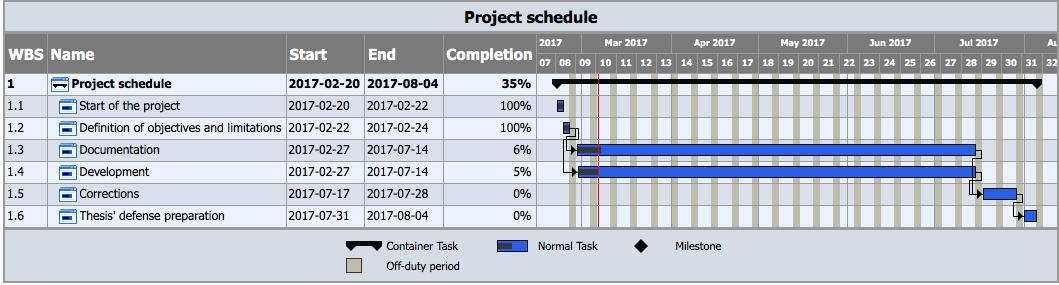
\includegraphics[width=.9\linewidth]{./images/project_schedule.png}
\caption{\label{fig:schedule}
The project's schedule.}
\end{figure}

Figure \ref{fig:schedule} shows the project's schedule.

\subsection{Literate programming}
\label{sec:org5f2f7a9}

This thesis' implementation is done by a procedure named ``literate
programming'', invented by Donald Knuth. What this means, is that the
documentation as well as the code for the resulting program reside in the same
file. The documentation is then \emph{weaved} into a separate document, which may be
any by the editor support format. The code of the program is \emph{tangled} into a
run-able computer program.

\begin{center}
\fbox{
\begin{minipage}[c]{.6\textwidth}
\textbf{\textsf{\textsc{TODO}}} Provide more information about literate programming.

\rule[.8em]{\textwidth}{2pt}

Citations, explain fragments, explain referencing
fragments, code structure does not have to be ``normal''
\end{minipage}
}
\end{center}

Originally it was planned to develop this thesis' application test driven,
providing (unit-) test-cases first and implementing the functionality
afterwards. Initial trails showed quickly that this method, in company with
literate programming, would exaggerate the effort needed. Therefore conventional
testing is used. Test are developed after implementing functionality and run
separately. A coverage as high as possible is intended. Test cases are \emph{tangled}
too, and may be found in the appendix.
\begin{center}
\fbox{
\begin{minipage}[c]{.6\textwidth}
\textbf{\textsf{\textsc{TODO}}} Insert reference/link to test cases here.

\end{minipage}
}
\end{center}

\section{Standards and principles}
\label{sec:org1f97866}
\subsection{Code}
\label{sec:orga31c13f}

\subsubsection{{\bfseries\sffamily TODO} Principles}
\label{sec:org091fa38}

\begin{itemize}
\item Classes use camel case.
\item Folders / name-spaces use only small letters.
\item Methods are all small caps and use underscores as spaces.
\item Signals: do\_something
\item Slots: on\_something
\item Importing: \texttt{from Foo import Bar}\\
As the naming of the PyQt5 modules prefixes them by \emph{Qt}, it is very unlikely
to have naming conflicts with other modules. Therefore the import format
\texttt{from PyQt5 import [QtModuleName]} is used. This still provides a
(relatively) unique naming most probably without any conflicts but reduces the
effort when writing a bit. The import of system modules is therefore as
follows.
\end{itemize}

\subsubsection{Layering}
\label{sec:layering}
Concerning the architecture, a layered architecture is foreseen, as stated in
\cite[p. 38 ff.]{osterwalder_qde_2016}. A relaxed layered architecture leads to
low coupling, reduces dependencies and enhances cohesion as well as clarity.

As the architecture's core \hyperref[sec:components]{components} are all graphical, a graphical user
interface for those components is developed. As the their data shall be
exportable, it would be relatively tedious if the graphical user interface would
hold and control that data. Instead models and model-view separation are used.
Additionally controllers are introduced which act as workflow objects of the
\texttt{application} layer and interfere between the model and its view.

\begin{enumerate}
\item Model-View-Controller
\label{sec:org900db8b}

While models may be instantiated anywhere directly, this would although not
contribute to having clean code and sane data structures. Instead controllers,
lying within the \texttt{application} layer, will manage instances of models.
The instantiating may either be induced by the graphical user interface
or by the player when loading and playing exported animations.

A view may never contain model-data (coming from the \texttt{domain} layer)
directly, instead view models are used \cite{martin_fowler_presentation_2004}.

The behavior described above corresponds to the well-known model-view-controller
pattern expanded by view models.

As Qt is used as the core for the editor, it may be quite obvious to use Qt's
model/view programming practices, as described by
\footnote{\url{http://doc.qt.io/qt-5/model-view-programming.html}}. However, Qt combines
the controller and the view, meaning the view acts also as a controller while
still separating the storage of data. The editor application does not actually
store data (in a conventional way, e.g. using a database) but solely exports it.
Due to this circumstance the model-view-controller pattern is explicitly used,
as also stated in \cite[p. 38]{osterwalder_qde_2016}.

\begin{center}
\fbox{
\begin{minipage}[c]{.6\textwidth}
\textbf{\textsf{\textsc{TODO}}} Describe the exact process of communication between

\end{minipage}
}
\end{center}
\begin{center}
\fbox{
\begin{minipage}[c]{.6\textwidth}
ViewModel, Controller and Model.

\end{minipage}
}
\end{center}

To avoid coupling and therefore dependencies, signals and
slots\footnote{\url{http://doc.qt.io/qt-5/signalsandslots.html}} are used in terms of the
observer pattern to allow inter-object and inter-layer communication.
\end{enumerate}

\subsubsection{Framework for implementation}
\label{sec:framework-for-implementation}
To stay consistent when implementing classes, it make sense to define a rough
framework for implementation, which is as follows:

\begin{enumerate}
\item Define necessary signals.
\item Within the constructor,
\begin{itemize}
\item Set up the user interface when it is a class concerning the graphical user
interface.
\item Set up class-specific aspects, such as the name, the tile or an icon.
\item Set up other components, used by that class.
\item Initialize the connections, meaning hooking up the defined signals with
corresponding methods.
\end{itemize}
\item Implement the remaining functionality in terms of methods and slots.
\end{enumerate}

\subsection{Diagrams}
\label{sec:orge6e23d9}

[Diagrams.]

\subsection{Project structure}
\label{sec:org2a3c2ff}

[Project structure.]
\chapter{{\bfseries\sffamily TODO} Implementation}
\label{sec:org0ebd240}
\section{Requirements}
\label{sec:org91530d8}
\subsection{Requirements}
\label{sec:orgbeafc3b}

This chapter describes the requirements to extract the source code out of this
documentation using \emph{tangling}.

At the current point of time, the requirements are the following:

\begin{itemize}
\item A Unix derivative as operating system (Linux, macOS).
\item Python version 3.5.x or up\footnote{\url{https://www.python.org}}.
\item Pyenv\footnote{\url{https://github.com/yyuu/pyenv}}.
\item Pyenv-virtualenv\footnote{\url{https://github.com/yyuu/pyenv-virtualenv}}.
\end{itemize}

The first step is to install a matching version of python for the usage within
the virtual environment. The available Python versions may be listed as follows.

\begin{listing}[H]
\begin{minted}[,fontsize=\footnotesize,linenos,bgcolor=bashcodebg]{bash}
pyenv install --list
\end{minted}
\caption{\label{fig:impl-pyenv-list}
Listing all available versions of Python for use in Pyenv.}
\end{listing}

The desired version may be installed as follows. This example shows the
installation of version 3.6.0.

\begin{listing}[H]
\begin{minted}[,fontsize=\footnotesize,linenos,bgcolor=bashcodebg]{bash}
install 3.6.0
\end{minted}
\caption{\label{fig:impl-pyenv-install}
Installation of Python version 3.6.0 for the usage with Pyenv.}
\end{listing}

It is highly recommended to create and use a project-specific virtual Python
environment. All packages, that are required for this project are installed
within this virtual environment protecting the operating systems' Python
packages.
First the desired version of Python has to be specified, then the desired name
of the virtual environment.

\begin{listing}[H]
\begin{minted}[,fontsize=\footnotesize,linenos,bgcolor=bashcodebg]{bash}
pyenv virtualenv 3.6.0 qde
\end{minted}
\caption{\label{fig:impl-pyenv-venv}
Creation of the virtual environment \texttt{qde} for Python using version 3.6.0 of Python.}
\end{listing}

All required dependencies for the project may now safely be installed. Those are
listed in the file \texttt{python\_requirements.txt} and are installed using \texttt{pip}.

\begin{listing}[H]
\begin{minted}[,fontsize=\footnotesize,linenos,bgcolor=bashcodebg]{bash}
pip install -r python_requirements.txt
\end{minted}
\caption{\label{fig:impl-pip-install}
Installation of the projects' required dependencies.}
\end{listing}

All requirements and dependencies are now met and the actual implementation of
the project may begin now.
\section{Name-spaces and project structure}
\label{sec:org0a653e7}
This chapter describes the planned directory structure as well as how the usage
of name-spaces is intended.

The whole source code shall be placed in the \texttt{src} directory underneath the main
directory. The creation of the single directories is not explicitly shown
respectively done, instead the \texttt{:mkdirp} option provided by the source code
block structure is used\footnote{\url{http://orgmode.org/manual/mkdirp.html\#mkdirp}}. The
option has the same effect as would have \texttt{mkdir -p [directory/subdirectory]}: It
creates all needed (sub-) directories, even when tangling a file. This prevents
the tedious and non-interesting creation of directories within this document.

When dealing with directories and files, Python uses the term \emph{package} for a
(sub-) directories and \emph{module} for files within directories, that is
modules.\footnote{\url{https://docs.python.org/3/reference/import.html\#packages}}

To prevent having multiple modules having the same name, name-spaces are
used\footnote{\url{https://docs.python.org/3/tutorial/classes.html\#python-scopes-and-namespaces}}.
The main name-space shall be analogous to the projects' name: \texttt{qde}. Underneath
the source code folder \texttt{src}, each sub-folder represents a package and acts
therefore also as a name-space.

To actually allow a whole package and its modules being imported \emph{as modules},
it needs to have at least a file inside called \texttt{\_\_init\_\_.py}. Those files may be
empty or they may contain regular source code such as classes or methods.

The first stage of the project shows the creation of the \emph{editor} component, as
it provides the possibility of creating and editing real-time animations which
may then be played back by the \emph{player} component\cite[p. 29]{osterwalder_qde_2016}.
\section{Editor}
\label{sec:orgfac95f1}
This chapter describes the creation of the \emph{editor} component.

The \emph{editor} component shall be placed within the \texttt{editor} directory beneath the
\texttt{src/qde} directory tree. As stated in the prior chapter this requires as well
an \texttt{\_\_init\_\_.py} file to let Python recognize the \texttt{editor} directory as a
importable module. This fact and the creation of it is mentioned here for the
sake of completeness. Later on it will be assumed as given and only the source
code blocks for the creation of the \texttt{\_\_init\_\_.py} files are provided.
\subsection{{\bfseries\sffamily DONE} Main application}
\label{sec:org57dd000}
\subsubsection{{\bfseries\sffamily DONE} Main application}
\label{sec:orgdb440f9}
The main class of a Qt application using a graphical user interface (GUI)
is provided by the class \texttt{QApplication}. According to
\footnote{\url{http://doc.qt.io/Qt-5/qapplication.html}} the class may be initialized and
used directly without sub-classing it. It may however be useful to sub-class it
nevertheless as this provides higher flexibility. Therefore the class
\texttt{Application} is introduced, which sub-classes the \texttt{QApplication} class.

At this point it is necessary to think about the functionality of the class
\texttt{Application} itself. Very roughly sketched, such a type of application
initializes resources, enters a main loop where it stays until told to shut
down. At the end it frees resources again.

Due to the usage of \texttt{QApplication} as super class it is not necessary to
implement a main (event-) loop, as such is provided by Qt itself
\footnote{\url{http://doc.qt.io/Qt-5/qapplication.html\#exec}}.

Concerning the initialization of
resources\footnote{\url{https://www.python.org/dev/peps/pep-0263/}}, the application has
to act as central node between the various layers of the architecture,
initializing them and connecting them using signals.\cite[S. 37 bis 38]{osterwalder_qde_2016}

Before going into too much details about the actual \texttt{Application} class, let us
first have a look at the structure of a Python module. Each (proper) Python
module contains an (optional) file encoding, a
docstring\footnote{\url{https://www.python.org/dev/peps/pep-0257/\#what-is-a-docstring}},
imports of other modules and either loose methods or a class definition with
methods underneath.

The main module \texttt{application} containing also the \texttt{Application} class, looks
therefore as follows.

\begin{listing}[H]
\begin{minted}[,fontsize=\footnotesize,linenos,bgcolor=bashcodebg]{python}
#!/usr/bin/python
# -*- coding: utf-8 -*-

"""Main application module for QDE."""

<<app-application-imports>>

<<app-application-class-definition>>
\end{minted}
\caption{Main application module holding the \texttt{Application} class.}
\end{listing}

\begin{enumerate}
\item Imports
\label{sec:org3721374}
As you can see, the imports of the module are defined by \texttt{<<app-application-imports>>}. For
achieving better readability, the imports are split up into system imports,
meaning modules provided by the Python library itself or external modules, and
project imports, modules created within the project. The imports are therefore
split up as follows.

\begin{listing}[H]
\begin{minted}[,fontsize=\footnotesize,linenos,bgcolor=bashcodebg]{python}
# System imports
<<app-application-system-imports>>

# Project imports
<<app-application-project-imports>>
\end{minted}
\caption{\label{app-application-imports}
\texttt{<<app-application-imports>>}, definition of the application modules' imports.}
\end{listing}

As the actual imports are not known yet, let us first look at the applications'
structure, defined by \texttt{<<app-class-definition>>}. The class is defined by its
name, its super class (the parent class) and a class body. As stated at the
beginning, the class will inherit from the Qt class \texttt{QApplication}, which
provides the basics for a Qt GUI application.

\begin{listing}[H]
\begin{minted}[,fontsize=\footnotesize,linenos,bgcolor=bashcodebg]{python}
class Application(QtWidgets.QApplication):
    """Main application for QDE."""

    <<app-application-class-body>>
\end{minted}
\caption{\label{app-application-class-definition}
\texttt{<<app-application-class-definition>>}, definition of the \texttt{Application} class.}
\end{listing}

As stated before and as clearly can be seen the class inherits from
\texttt{QApplication}. This base class is not yet defined however which would produce
an error when executing the main class. It is therefore necessary to make that
base class available by importing it. As \texttt{QApplication} is an external class,
not defined by this project, its import is added to the system imports.

Python offers multiple possibilities concerning imports:

\begin{itemize}
\item \texttt{from foo import bar} or\\
\texttt{import foo.bar}

Imports the module \texttt{bar} from the package \texttt{foo}. All classes, methods and
variables within \texttt{bar} are then accessible.

\item \texttt{from foo import bar as baz} or\\
\texttt{import foo.bar as baz}

The importing is the same as above, \texttt{bar} is masked as \texttt{baz} although. This
can be convenient when multiple modules have the same name.

\item \texttt{from bar import SomeClass} or\\
\texttt{import bar.SomeClass} or\\
\texttt{import bar.SomeClass as SomeClass}

Imports the class \texttt{SomeClass} from the module \texttt{bar}.

\item \texttt{from foo.bar import some\_method} or\\
\texttt{import foo.bar.some\_method} or\\
\texttt{import foo.bar.some\_method as some\_method}

Imports the method \texttt{some\_method} from the module \texttt{bar}.

\item \texttt{from foo import *} or\\
\texttt{import * from foo}

Imports \emph{all} sub-packages and sub-modules from the package \texttt{foo}. However,
explicit importing is better than implicit and therefore this option should
not be used.\footnote{\url{https://www.python.org/dev/peps/pep-0020/}}

\item \texttt{from bar import *} or
\texttt{import * from bar}

Imports \emph{all} classes and methods from the module \texttt{bar}. As stated above,
explicit importing is better than implicit and therefore this option should
also not be used.
\end{itemize}

As the naming of the PyQt5 modules prefixes them by \emph{Qt}, it is very unlikely to
have naming conflicts with other modules. Therefore the import format \texttt{from
PyQt5 import [QtModuleName]} is used. This still provides a (relatively) unique
naming most probably without any conflicts but reduces the effort when
writing a bit. The import of system modules is therefore as follows.

\begin{listing}[H]
\begin{minted}[,fontsize=\footnotesize,linenos,bgcolor=bashcodebg]{python}
from PyQt5 import QtGui
from PyQt5 import QtWidgets
\end{minted}
\caption{\label{app-application-system-imports}
\texttt{<<app-application-system-imports>>}, import of system imports.}
\end{listing}

At this point of time it is rather unclear what the classes body consists of.
What surely must be done, is initializing the class's parent, \texttt{QApplication}.
Additionally it would be nice to having a matching title for the window set as
well as maybe an icon for the application. The class's body therefore solely
consists its constructor, as follows.

\begin{listing}[H]
\begin{minted}[,fontsize=\footnotesize,linenos,bgcolor=bashcodebg]{python}
<<app-application-constructor>>

def setup_components(self):
    <<app-application-methods-setup-components>>

def setup_connections(self):
    <<app-application-methods-setup-connections>>

<<app-application-methods>>
\end{minted}
\caption{\label{app-application-class-body}
\texttt{<<app-application-class-body>>}, body of the class \texttt{Application}, containing only the constructor at the moment.}
\end{listing}

When looking at the constructor of the \texttt{QApplication}
class\footnote{\url{https://doc.qt.io/qt-5/qapplication.html\#QApplication}} (as the
documentation of PyQt does not provide a proper description and points to the
C++ documentation), one can see that it needs the argument count \texttt{argc} as well
as a vector \texttt{argv} containing the arguments. The argument count states how many
arguments are being held by the argument vector \texttt{argv}. In the PyQt
implementation however, only one argument is necessary: a list containing the
arguments. \texttt{argc} may easily be derived by e.g. \texttt{len(arguments)}. Therefore it
is necessary for to constructor to take in \texttt{arguments} as a required parameter.
As described in section \ref{sec:framework-for-implementation}, a method for setting up
the connections, which may be defined later on, is added to the constructor. The
application's constructor looks hence as follows.

\begin{listing}[H]
\begin{minted}[,fontsize=\footnotesize,linenos,bgcolor=bashcodebg]{python}
def __init__(self, arguments):
    """Constructor.

    :param arguments: a (variable) list of arguments, that are
                      passed when calling this class.
    :type  argv:      list
    """

    super(Application, self).__init__(arguments)
    self.setWindowIcon(QtGui.QIcon("assets/icons/im.png"))
    self.setApplicationName("QDE")
    self.setApplicationDisplayName("QDE")

    self.setup_components()
    self.setup_connections()
\end{minted}
\caption{\label{app-application-constructor}
\texttt{<<app-application-constructor>>}, constructor of the \texttt{Application} class.}
\end{listing}
\end{enumerate}
\subsection{{\bfseries\sffamily DONE} Main entry point}
\label{sec:orgfffe376}
\subsubsection{{\bfseries\sffamily DONE} Main entry point}
\label{sec:org2a4c7a6}
If you run the application at this point nothing happens. Python is able to
resolve all dependencies but as there is no \texttt{main} function there is nothing
else to do, so nothing happens. The execution of the main loop is started when
calling the \texttt{exec} function of a \texttt{QApplication}. So, for actually being able to
start the application, a \texttt{main} function is needed, which creates an instance of
the \texttt{Application} class and then runs its \texttt{exec} function.

The main function could easily be added to the \texttt{Application} class, but for
somebody who is not familiar with this applications' structure, this might be
rather confusing. Instead a \texttt{editor.py} file at the root of the source directory
\texttt{src} is much more intuitive.

All that the main file shall do, is creating an instance of the main
application, execute it and exit at the end of its life cycle.

As stated in \label{Imports}, the constructor of \texttt{QApplication} requires the
argument \texttt{arguments} to be passed in (yes, the naming may be a bit confusing
here). The \texttt{arguments} argument is a list of arguments passed when calling the
main entry point of the editor application. For example when calling \texttt{python editor.py foo bar baz},
the variable \texttt{arguments} would be the list \texttt{[foo, bar, baz]} with
\texttt{len(arguments)} being 3. To obtain the passed-in arguments, the \texttt{argv}
attribute of the \texttt{sys} module may be used, as this holds exactly the list of the
passed-in arguments when calling a Python script.

The main entry script of the editor \texttt{editor.py} is therefore defined as follows.

\begin{listing}[H]
\begin{minted}[,fontsize=\footnotesize,linenos,bgcolor=bashcodebg]{python}
#!/usr/bin/python
# -*- coding: utf-8 -*-

""" Main entry point for the QDE editor application. """

# System imports
import sys

# Project imports
from qde.editor.application import application


if __name__ == "__main__":
    app = application.Application(sys.argv)
    status = app.exec()
    sys.exit(status)
\end{minted}
\caption{\label{main}
\texttt{<<main>>}, the main entry point for the whole editor application.}
\end{listing}

If you run the application now, a bit more happens. Python is able to
resolve all dependencies and to find a \texttt{main} function which is then called.
The \texttt{main} function creates an instance of the \texttt{Application} class and executes
it by calling \texttt{exec}. This in turn enters the Qt main loop which keeps the
application running unless explicitly told to shut down. But at this point there
is nothing who could receive the request to shut down, so the only possibility
to shut down the application is to quit or kill the spawned Python process
itself --- not very nice.
\subsection{{\bfseries\sffamily DONE} Components}
\label{sec:components}
Instead it would be nice to have at least a window shown when starting the
application, which allows a normal, deterministic and convenient shut down of
the application, either by a keyboard shortcut or by selecting an appropriate
option in the applications' menu.

But having only a plain window is not that interesting, so this might be a good
time to look at the components of the editor, which are defined by
\citep[p. 29 ff.]{osterwalder_qde_2016} and are the following:

\begin{itemize}
\item A scene graph, allowing the creation and deletion of scenes. The scene graph
has at least a root scene.
\item A node-based graph structure, allowing the composition of scenes using nodes
and connections between the nodes.
\item A parameter window, showing parameters of the currently selected graph node.
\item A rendering window, rendering the currently selected node or scene.
\item A sequencer, allowing a time-based scheduling of defined scenes.
\end{itemize}

What \cite{osterwalder_qde_2016} does not explicitly mention, is the main
window, which holds all those components and allows a proper shut down of the
application.

As a starting point, we shall implement the class \texttt{MainWindow}
representing the main window.
\subsection{{\bfseries\sffamily TODO} Main window}
\label{sec:org8e1c2da}
\subsubsection{{\bfseries\sffamily TODO} Main window}
\label{sec:orgc7b6788}

Before implementing the features of the main window, its features will be
described. The main window is the central aspect of the graphical user interface
and is hence part of the \texttt{gui} package.

Its main functionality is to set up the actual user interface, containing all
the components, described by \ref{sec:components}, as widgets. Qt offers the class
\texttt{QMainWindow} from which \texttt{MainWindow} may inherit. The thoughts about the
implementation follow section \ref{sec:framework-for-implementation}.

The first step is setting up the necessary signals. They may not all be known at
this point and may therefore be expanded later on. As described in section
\ref{sec:components}, it would be nice if \texttt{MainWindow} would react to a request for
closing it, either by a keyboard shortcut or a menu command. However,
\texttt{MainWindow} is not able to force the \texttt{Application} to quit by itself. It would
be possible to pass \texttt{MainWindow} a reference to \texttt{Application} but that would
lead to a somewhat tight coupling and is therefore not considered as an option.
Signals and slots allow exactly such cross-layer communication without coupling
components tightly.

First, the outline of \texttt{MainWindow} is defined.

\begin{listing}[H]
\begin{minted}[,fontsize=\footnotesize,linenos,bgcolor=bashcodebg]{python}
#!/usr/bin/python
# -*- coding: utf-8 -*-

""" Module holding the main application window. """

# System imports
<<main-window-system-imports>>

# Project imports
<<main-window-project-imports>>


class MainWindow(QtWidgets.QMainWindow):
    """The main window class.
    Acts as an entry point for the QDE editor application.
    """

    <<main-window-signals>>

    def __init__(self):
        """Constructor."""

        <<main-window-constructor>>

    <<main-window-methods>>

    <<main-window-slots>>
\end{minted}
\caption{Module holding the main application window class, \texttt{MainWindow}.}
\end{listing}

A fitting name for the signal, when the window and therefore the application,
shall be closed might be \texttt{window\_closing}. The signal is introduced as follows.

\begin{listing}[H]
\begin{minted}[,fontsize=\footnotesize,linenos,bgcolor=bashcodebg]{python}
# Signals
window_closing = QtCore.pyqtSignal()
\end{minted}
\caption{\label{main-window-signals}
Definition of signals for the main application window class, \texttt{MainWindow}.}
\end{listing}

Now, that the signal for closing the window and the application is defined, two
additional things need to be considered: The emission of the signal by
\texttt{MainWindow} itself as well as the consumption of the signal by a slots of other
classes.

First, the emission of the signal is implemented. The signal shall be emitted
when the escape key on the keyboard is pressed or when the corresponding menu
item was selected. For the first case, the keyboard event, Qt provides luckily
events which may be used. Their outline is already provided by the parent class
\texttt{QMainWindow} and therefore the event(s) simply need to be implemented. The
event which listens to keyboard keys being pressed is called \texttt{keyPressEvent} and
provides an event-object of type \texttt{QEvent}. All there is to do, is to retrieve
the event's key by calling its \texttt{key} method and check if that key is actually
the escape key by comparing it to \texttt{Key\_Escape}, provided by Qt. If this
comparison is true, the signal shall be emitted.

\begin{listing}[H]
\begin{minted}[,fontsize=\footnotesize,linenos,bgcolor=bashcodebg]{python}
def keyPressEvent(self, event):
    """Gets triggered when a key press event is raised.

    :param event: holds the triggered event.
    :type  event: QKeyEvent
    """

    if event.key() == QtCore.Qt.Key_Escape:
        self.window_closing.emit()
    else:
        super(MainWindow, self).keyPressEvent(event)
\end{minted}
\caption{\label{main-window-keypressevent}
Implementation of the \texttt{keyPressEvent} method on the \texttt{MainWindow} class.}
\end{listing}

Additionally the signal shall be emitted when selecting a corresponding menu
item. But currently there is no such menu item defined. Qt handles interactions
with menu items by using actions (\texttt{QAction}). They provide themselves a couple
of signals, one being \texttt{triggered}, which gets emitted as soon as the action was
triggered by a clicking on a menu item. As it is not possible to connect a
signal with another signal, a slot, which receives the signal, needs to be
defined. A slot is an annotated method.

\begin{listing}[H]
\begin{minted}[,fontsize=\footnotesize,linenos,bgcolor=bashcodebg]{python}
@QtCore.pyqtSlot()
def on_quit(self):
    """Slot which emits the :any:`window_closing` signal.
    This slot gets triggered upon the selection of the menu item to close the
    QDE application.
    """

    self.window_closing.emit()
\end{minted}
\caption{\label{main-window-slots}
The \texttt{on\_quit} method, which acts as a slot when the menu item for quitting the application was triggered.}
\end{listing}

Now the main window is able to emit the signal it is shutting down (or
rather it would like to shut down), but so far no one is listening to that
signal, so nothing happens when that signal is being emitted.

This leads to an expansion of the main application's construction: The main
application has to create a main window an listen to its \texttt{window\_closing}
signal. Luckily \texttt{Application} provides already a \texttt{quit} slot through
\texttt{QApplication}.

\begin{listing}[H]
\begin{minted}[,fontsize=\footnotesize,linenos,bgcolor=bashcodebg]{python}
self.main_window = qde_main_window.MainWindow()
self.main_window.window_closing.connect(self.quit)
\end{minted}
\caption{\label{app-application-methods-setup-components}
Expansion of setting up the main application's components by the initialization of \texttt{MainWindow} and its signals.}
\end{listing}

So far none of the additional modules have been defined as there are no
additional modules imported yet. The missing modules need to be added to the
main application as well as the main window.

\begin{listing}[H]
\begin{minted}[,fontsize=\footnotesize,linenos,bgcolor=bashcodebg]{python}
from qde.editor.gui import main_window as qde_main_window
\end{minted}
\caption{\label{app-application-project-imports}
Expansion of \texttt{<<app-application-project-imports>>} by the missing imports.}
\end{listing}

\begin{listing}[H]
\begin{minted}[,fontsize=\footnotesize,linenos,bgcolor=bashcodebg]{python}
from PyQt5 import QtCore
from PyQt5 import QtWidgets
\end{minted}
\caption{\label{main-window-system-imports}
Expansion of \texttt{<<main-window-system-imports>>} by the missing imports.}
\end{listing}

Yet the constructor for the main window is still missing, so running the
application would still do nothing. Therefore the constructor for the main
window is now implemented. At the current point its solely purpose is to call
the its parent's constructor.

\begin{listing}[H]
\begin{minted}[,fontsize=\footnotesize,linenos,bgcolor=bashcodebg]{python}
super(MainWindow, self).__init__()
\end{minted}
\caption{\label{main-window-constructor}
Constructor for the main window class \texttt{MainWindow}.}
\end{listing}

Although a Python process is spawned when starting the application, the main
window is still not shown. The problem is, that the main window has no central
widget
set\footnote{\url{http://doc.qt.io/qt-5/qmainwindow.html\#creating-main-window-components}}.
Setting a central widget and setting a layout for it solves this problem.

The above described task matches perfectly the second point described in section
\ref{sec:framework-for-implementation}. The described task will therefore be put in a
method named \texttt{setup\_ui} and the constructor will be expanded correspondingly.
The method \texttt{setup\_ui} seems also a very good place for setting things like the
size of the window, setting its (object-) name and its title as well as moving
it to a position on the user's screen. To ensure that the window is not hidden
behind other windows, the method \texttt{activateWindow} coming from \texttt{QWidget} is
called.

As it is not sure at this point, if the main window will receive additional
methods, it may be wise to split \texttt{<<main-window-methods>>} up, by inserting the
yet known methods (only \texttt{setup\_ui} so far) explicitly. This provides the
advantage, that new methods can easily be appended and the implemented methods
may be expanded easily as well.

\begin{listing}[H]
\begin{minted}[,fontsize=\footnotesize,linenos,bgcolor=bashcodebg]{python}
<<main-window-keypressevent>>

<<main-window-setupui>>
\end{minted}
\caption{\label{main-window-methods}
The placeholder \texttt{<<main-window-methods>>} declared explicitly.}
\end{listing}

\begin{listing}[H]
\begin{minted}[,fontsize=\footnotesize,linenos,bgcolor=bashcodebg]{python}
def setup_ui(self):
    """Sets up the user interface specific components."""

    self.setObjectName('MainWindow')
    self.setWindowTitle('QDE')
    self.resize(1024, 768)
    self.move(100, 100)
    self.activateWindow()

    central_widget = QtWidgets.QWidget(self)
    central_widget.setObjectName('central_widget')
    grid_layout = QtWidgets.QGridLayout(central_widget)
    central_widget.setLayout(grid_layout)
    self.setCentralWidget(central_widget)
    self.statusBar().showMessage('Ready.')
\end{minted}
\caption{\label{main-window-setupui}
The method \texttt{setup\_ui}, which was added to \texttt{<<main-window-methods>> before, for setting up user interface specific tasks within the main window class =MainWindow}.}
\end{listing}

Now the \texttt{setup\_ui} method simply needs to be added to the constructor of the
class \texttt{MainWindow}.

\begin{listing}[H]
\begin{minted}[,fontsize=\footnotesize,linenos,bgcolor=bashcodebg]{python}
self.setup_ui()
\end{minted}
\caption{\label{main-window-constructor}
The method \texttt{setup\_ui} is added to the constructor of main window class \texttt{MainWindow}.}
\end{listing}

Finally the main window has to be shown by calling its \texttt{show} method
at the end of the main application's construction.

\begin{listing}[H]
\begin{minted}[,fontsize=\footnotesize,linenos,bgcolor=bashcodebg]{python}
    self.main_window.show()
\end{minted}
\caption{\label{app-application-constructor}
The main window is being shown at the end of the main application's construction.}
\end{listing}

\begin{figure}[H]
\centering
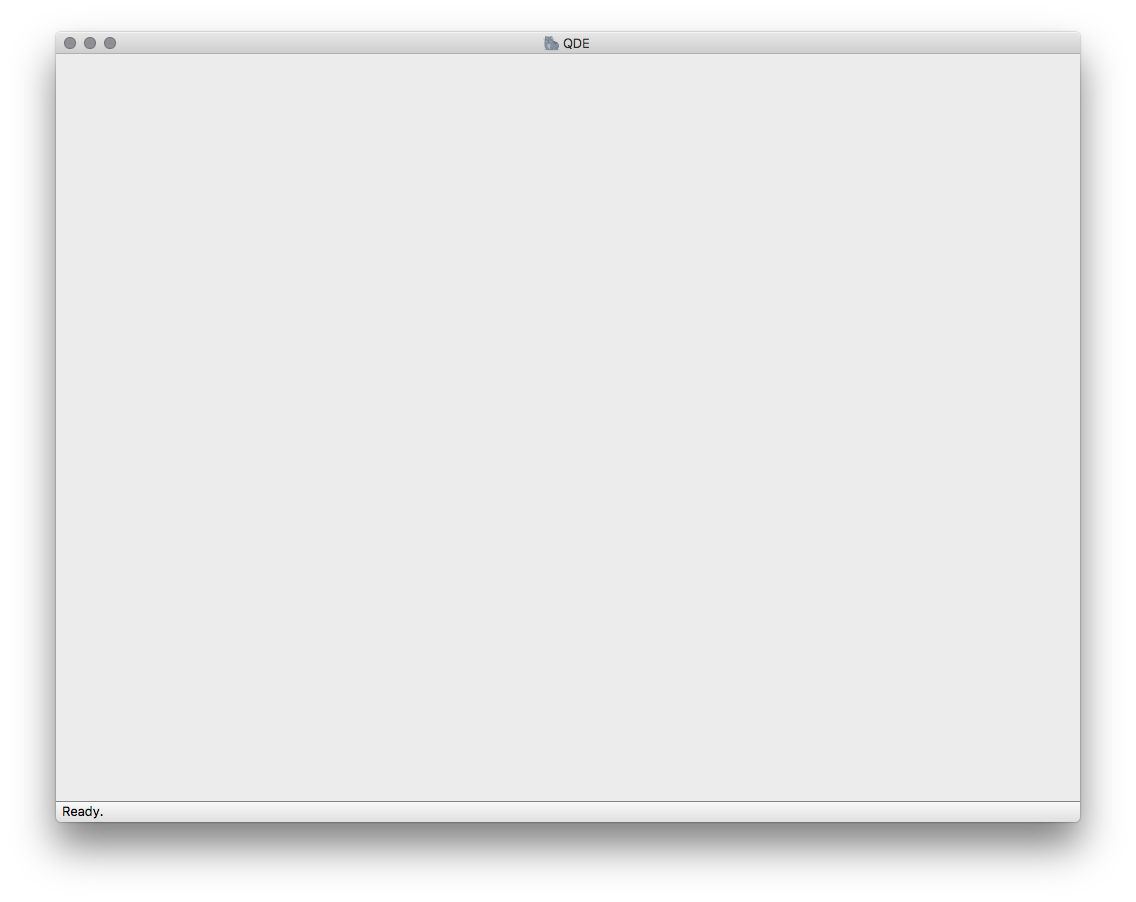
\includegraphics[width=0.5\textwidth]{./images/qde_alpha_01.png}
\caption{\label{fig:editor-alpha-01}
The QDE editor application in a very early stage, containing only a grid layout.}
\end{figure}

When starting the application a plain window containing a grid layout is shown,
as can be seen in figure \ref{fig:editor-alpha-01}. As written in \ref{sec:components} and
shown in \citep[p. 29 ff.]{osterwalder_qde_2016}, the main window will contain all
the components. To ensure, that those components are shown as defined, a simple
grid layout may not provide enough possibilities.

A possible solution to reach the desired layout is to use the horizontal box
layout \texttt{QHBoxLayout} in combination with splitters. The horizontal box layout
lines up widgets horizontally where as the splitters allow splitting either
horizontally or vertically. Recalling the components from \ref{sec:components}, the following are needed:

\begin{itemize}
\item A scene graph, on the left of the window, covering the whole height
\item A node graph on the right of the scene graph, covering as much height as
possible
\item A view for showing the properties (and therefore parameters) of the selected
node on the right of the node graph, covering as much height as possible
\item A display for rendering the selected node, on the right of the properties
view, covering as much height as possible
\item A sequencer at the right of the scene graph and below the other components at
the bottom of the window, covering as much width as possible
\end{itemize}

To sum up, a horizontally box layout and a vertical splitter allow splitting the
main window in two halves: The left side will be used for the scene graph where
as the other side will hold the remaining components. As the sequencer is
located below the other components of the right side, a horizontal splitter is
needed for proper separation. The components above the sequencer could simply be
added to the right side of the split as a horizontal box layout builds the
layout's basis, for convenience however, additional splitters will be used. This
allows the user to re-arrange the layout to his taste. To achieve the described
layout, the following tasks are necessary:

\begin{itemize}
\item Create a widget for the horizontal box layout
\item Create the horizontal box layout
\item Add the scene graph to the horizontal box layout
\item Instantiate the components of the split's right side
\begin{itemize}
\item The node graph
\item The parameter view
\item The rendering view
\end{itemize}
\item Create a horizontal splitter
\begin{itemize}
\item Add the rendering view to it
\item Add the parameter view to it
\end{itemize}
\item Create a vertical splitter
\begin{itemize}
\item Add the horizontally splitter to it
\item Add the scene graph to it
\end{itemize}
\item Add the vertical splitter to the horizontal box layout
\end{itemize}

The implementation of the explained layout is done in the \texttt{setup\_ui} method and
is as follows. For the not yet existing widgets placeholders are used.

\begin{listing}[H]
\begin{minted}[,fontsize=\footnotesize,linenos,bgcolor=bashcodebg]{python}
    horizontal_layout_widget = QtWidgets.QWidget(central_widget)
    horizontal_layout_widget.setObjectName('horizontal_layout_widget')
    horizontal_layout_widget.setGeometry(QtCore.QRect(12, 12, 781, 541))
    horizontal_layout_widget.setSizePolicy(QtWidgets.QSizePolicy.MinimumExpanding,
                                           QtWidgets.QSizePolicy.MinimumExpanding)
    grid_layout.addWidget(horizontal_layout_widget, 0, 0)

    horizontal_layout = QtWidgets.QHBoxLayout(horizontal_layout_widget)
    horizontal_layout.setObjectName('horizontal_layout')
    horizontal_layout.setContentsMargins(0, 0, 0, 0)

    <<main-window-setupui-scenegraph>>
    <<main-window-setupui-nodegraph>>
    <<main-window-setupui-parameterview>>
    <<main-window-setupui-renderview>>

    horizontal_splitter = QtWidgets.QSplitter()
    <<main-window-setupui-add-renderview-to-horizontal-splitter>>
    <<main-window-setupui-add-parameterview-to-horizontal-splitter>>

    vertical_splitter = QtWidgets.QSplitter()
    vertical_splitter.setOrientation(QtCore.Qt.Vertical)
    vertical_splitter.addWidget(horizontal_splitter)
    <<main-window-setupui-add-nodegraph-to-vertical-splitter>>

    horizontal_layout.addWidget(vertical_splitter)
\end{minted}
\caption{\label{main-window-setupui}
Lay-outing of the main window by expanding the \texttt{setup\_ui} method.}
\end{listing}

All the above taken actions to lay out the main window change nothing in the
window's yet plain appearance. This is quite obvious, as none of the actual
components are implemented yet.

The most straight-forward component to implement may be scene graph, so this is
a good starting point for the implementation of the remaining components.
\subsection{{\bfseries\sffamily DONE} Scene graph}
\label{sec:org5cb8369}
\subsubsection{{\bfseries\sffamily DONE} Scene graph}
\label{sec:org0e05964}
The scene graph component does, as also the other components do, have two
aspects to consider: A graphical aspect as well as its data structure. As
written in section \ref{sec:layering}, each component has a view --- residing in the \emph{gui}
package ---, a model --- residing in the \emph{domain} package --- and a controller
acting as workflow object --- residing in the \emph{application} package.

The \texttt{SceneGraphController} class will manage instances of scene models
whereas the \texttt{SceneGraphView} will display a tree of scenes, starting
with a root scene of type \texttt{SceneModel}.

The least tedious of those aspects may be the scene model, \texttt{SceneModel}, so
the scene model is implemented first.

As at this point its functionality is not known, its implementation is rather
dull. It is composed of solely an empty constructor.

\begin{listing}[H]
\begin{minted}[,fontsize=\footnotesize,linenos,bgcolor=bashcodebg]{python}
#!/usr/bin/python
# -*- coding: utf-8 -*-

""" Module holding scene related aspects concerning the domain layer. """

# System imports
<<domain-scene-system-imports>>

# Project imports
<<domain-scene-project-imports>>


class SceneModel(object):
    """The scene model.
    It is used as a base class for scene instances within the scene graph.
    """

    <<domain-scene-signals>>

    <<domain-scene-constructor>>

    <<domain-scene-methods>>

    <<domain-scene-slots>>
\end{minted}
\caption{Scene module inside the \texttt{domain} package, holding the \texttt{SceneModel} class.}
\end{listing}

\begin{listing}[H]
\begin{minted}[,fontsize=\footnotesize,linenos,bgcolor=bashcodebg]{python}
def __init__(self):
    pass
\end{minted}
\caption{\label{domain-scene-constructor}
Constructor of the scene model class, \texttt{SceneModel}.}
\end{listing}

Scenes may now be instantiated, it is however important to do the management of
scenes in a controlled manner. This is where the specific controllers within the
\texttt{application} layer come in, as described in more detail in section
\ref{sec:layering}. Therefore the class \texttt{SceneGraphController} will now be
implemented, for being able to manage scenes.

As the scene graph shall be built as a tree structure, an appropriate data
structure is needed. Qt provides the \texttt{QTreeWidget} class, but that
class is in this case not suitable, as it does not separate the data from its
representation, as stated by Qt: ``Developers who do not need the flexibility of
the Model/View framework can use this class to create simple hierarchical lists
very easily. A more flexible approach involves combining a QTreeView with a
standard item model. This allows the storage of data to be separated from its
representation.''\footnote{\url{http://doc.qt.io/qt-5/qtreewidget.html\#details}}

Therefore the class
\texttt{QAbstractItemModel}\footnote{\url{http://doc.qt.io/qt-5/qabstractitemmodel.html}}
is chosen for implementation. Before implementing the actual methods, it is
important to think about the attributes, that the scene graph controller will
have. According to the class's documentation, some methods must be implemented
at very least: ``When subclassing QAbstractItemModel, at the very least you must
implement index(), parent(), rowCount(), columnCount(), and data(). These
functions are used in all read-only models, and form the basis of editable
models.''

For being able edit the nodes of the scene graph and to have a custom header
displayed, further methods have to be implemented: ``To enable editing in your
model, you must also implement setData(), and reimplement flags() to ensure that
ItemIsEditable is returned. You can also reimplement headerData() and
setHeaderData() to control the way the headers for your model are presented.''

From the remarks above the attributes may be defined. As the scene graph is
implemented as a tree structure, it must have a \textbf{root node}, which is of type
\texttt{SceneGraphViewModel} (coming from the \texttt{gui\_domain} layer).
Whenever a scene is added as a node, the item model needs to be informed for
updating the display. This happens by emitting the \texttt{rowsInserted}
signal, which is already given by the \texttt{QAbstractItemModel} class. This
signal needs the current model index as well as the first and last position as
parameters. The current model index represents the parent of the item to add,
whereas the item will be inserted between the two given positions, first and
last. Concerning the model index the Qt documentation states: ``An invalid model
index can be constructed with the QModelIndex constructor. Invalid indexes are
often used as parent indexes when referring to top-level items in a model.''
Therefore for creating the initial node of the scene graph, the root node, the
constructor of \texttt{QModelIndex} will be used.
As \textbf{header data} the name of the scenes as well as the number of nodes a scene
contains shall be displayed.

Speaking of signals, brings up the definition of signals for the scene graph
controller. To prevent coupling, two signals are added: \texttt{scene\_added}
and \texttt{scene\_removed}. The first will be emitted whenever a new node is
inserted into the scene graph by \texttt{insertRows} being called. The latter
is emitted whenever an existing node is removed from the scene graph by calling
the \texttt{removeRows} method.

But what currently is missing for being able to implement a first draft of the
scene graph, is the view model \texttt{SceneGraphViewModel}. View models are
used to visually represent something within the graphical user interface and
they provide an interface to the \texttt{domain} layer. To this point, a
simple reference in terms of an attribute is used, which may be changed later
on. Concerning the user interface, a view model must fulfill the requirements
posed by the user interface's corresponding component. In terms of the scene
graph the view model must provide at least a name and a row. Additionally, as
already mentioned, a reference to the domain object is being added. The class
inherits from \texttt{QObject} as this base class already provides a tree
structure, which fits the structure of the scene graph perfectly.

\begin{listing}[H]
\begin{minted}[,fontsize=\footnotesize,linenos,bgcolor=bashcodebg]{python}
#!/usr/bin/python
# -*- coding: utf-8 -*-

""" Module holding scene related aspects concerning the gui_domain layer. """

# System imports
from PyQt5 import Qt
from PyQt5 import QtCore
<<guidomain-scene-system-imports>>

# Project imports
<<guidomain-scene-project-imports>>

<<guidomain-scene-body>>
\end{minted}
\caption{\label{guidomain-scene}
Scene module inside the \texttt{gui\_domain} package.}
\end{listing}

\begin{listing}[H]
\begin{minted}[,fontsize=\footnotesize,linenos,bgcolor=bashcodebg]{python}
<guidomain-scene-body>=
    class SceneGraphViewModel(Qt.QObject):
        """View model representing scene graph items.
    
        The SceneGraphViewModel corresponds to an entry within the scene graph. It
        is used by the QAbstractItemModel class and must therefore at least provide
        a name and a row.
        """
    
        
    
        # .. py:function::
        def __init__(
                self,
                row,
                domain_object,
                name=QtCore.QCoreApplication.translate('SceneGraphViewModel', 'New scene'),
                parent=None
        ):
            """Constructor.
        
            :param row:           The row the view model is in.
            :type  row:           int
            :param domain_object: Reference to a scene model.
            :type  domain_object: qde.editor.domain.scene.SceneModel
            :param name:          The name of the view model, which will be displayed in
                                  the scene graph.
            :type  name:          str
            :param parent:        The parent of the current view model within the scene
                                  graph.
            :type parent:         qde.editor.gui_domain.scene.SceneGraphViewModel
            """
        
            super(SceneGraphViewModel, self).__init__(parent)
            self.row  = row
            self.domain_object = domain_object
            self.name = name
            self.scene_view_model = SceneViewModel()
\end{minted}
\caption{\label{lst:guidomain-scene-scenegraphviewmodel}
Definition of the body of the \texttt{scene} module, which is in the \texttt{gui\_domain} layer.}
\end{listing}

\begin{listing}[H]
\begin{minted}[,fontsize=\footnotesize,linenos,bgcolor=bashcodebg]{python}
# .. py:function::
def __init__(
        self,
        row,
        domain_object,
        name=QtCore.QCoreApplication.translate('SceneGraphViewModel', 'New scene'),
        parent=None
):
    """Constructor.

    :param row:           The row the view model is in.
    :type  row:           int
    :param domain_object: Reference to a scene model.
    :type  domain_object: qde.editor.domain.scene.SceneModel
    :param name:          The name of the view model, which will be displayed in
                          the scene graph.
    :type  name:          str
    :param parent:        The parent of the current view model within the scene
                          graph.
    :type parent:         qde.editor.gui_domain.scene.SceneGraphViewModel
    """

    super(SceneGraphViewModel, self).__init__(parent)
    self.row  = row
    self.domain_object = domain_object
    self.name = name
\end{minted}
\caption{\label{guidomain-scene-scenegraphviewmodel-constructor}
Constructor for the scene graph view model, \texttt{SceneGraphViewModel}.}
\end{listing}

Now, with the scene graph view model being available, the scene graph controller
may finally be implemented.

\begin{listing}[H]
\begin{minted}[,fontsize=\footnotesize,linenos,bgcolor=bashcodebg]{python}
#!/usr/bin/python
# -*- coding: utf-8 -*-

""" Module holding scene graph related aspects concerning the application layer.
"""

# System imports
from PyQt5 import QtCore
<<app-scenegraph-system-imports>>

# Project imports
from qde.editor.domain     import scene as domain_scene
from qde.editor.gui_domain import scene as guidomain_scene
<<app-scenegraph-project-imports>>


class SceneGraphController(QtCore.QAbstractItemModel):
    """The scene graph controller.
    A controller for managing the scene graph by adding, editing and removing
    scenes.
    """

    scene_added = QtCore.pyqtSignal(domain_scene.SceneModel)
    scene_removed = QtCore.pyqtSignal(domain_scene.SceneModel)
    <<app-scenegraph-controller-signals>>

    def __init__(self, root_node_domain_object, parent=None):
        """Constructor.

        :param root_node_domain_object: The domain object of the root node of
                                        the scene graph view model.
        :type root_node_domain_object:  qde.editor.domain.scene.SceneModel
        :param parent: The parent of the current view model within the scene
                       graph.
        :type parent:  qde.editor.gui_domain.scene.SceneGraphViewModel
        """

        super(SceneGraphController, self).__init__(parent)
        self.header_data = [
            QtCore.QCoreApplication.translate(__class__.__name__, 'Name'),
            QtCore.QCoreApplication.translate(__class__.__name__, '# Nodes')
        ]
        self.root_node = guidomain_scene.SceneGraphViewModel(
            row=0,
            domain_object=root_node_domain_object,
            name=QtCore.QCoreApplication.translate(__class__.__name__, 'Root scene')
        )
        self.rowsInserted.emit(QtCore.QModelIndex(), 0, 1)
        <<app-scenegraph-controller-constructor>>

    <<app-scenegraph-controller-methods>>

    <<app-scenegraph-controller-slots>>
\end{minted}
\caption{\label{lst:app-scenegraph}
The outline of the \texttt{SceneGraphController} class, inside the \texttt{application} package.}
\end{listing}

At this point data structures in terms of a (data-) model, which holds the
actual, for the scene graph relevant data of a scene, and a view model, which
holds the data relevant for the user interface, are implemented. Further a
controller for handling the flow of the data for both models is implemented.
What is still missing, is the actual representation of the scene graph in terms
of a view.

Qt offers a plethora of widgets for implementing views. One such widget is
\texttt{QTreeView}, which ``implements a tree representation of items from a
model. This class is used to provide standard hierarchical lists that were
previously provided by the QListView class, but using the more flexible approach
provided by Qt's model/view
architecture.''\footnote{\url{http://doc.qt.io/qt-5/qtreeview.html\#details}}

\begin{listing}[H]
\begin{minted}[,fontsize=\footnotesize,linenos,bgcolor=bashcodebg]{python}
#!/usr/bin/python
# -*- coding: utf-8 -*-

""" Module holding scene related aspects concerning the graphical user interface layer.
"""

# System imports
from PyQt5 import QtWidgets
<<gui-scene-system-imports>>

# Project imports
<<gui-scene-project-imports>>


<<gui-scene-graph-class-decorators>>
class SceneGraphView(QtWidgets.QTreeView):
    """The scene graph view widget.
    A widget for displaying and managing the scene graph.
    """

    # Signals
    <<gui-scene-graph-signals>>

    def __init__(self, parent=None):
        """Constructor.

        :param parent:        The parent of the current view widget.
        :type parent:         QtCore.QObject
        """

        super(SceneGraphView, self).__init__(parent)
        <<gui-scene-graph-constructor>>

    <<gui-scene-graph-methods>>

    # Slots
    <<gui-scene-graph-slots>>
\end{minted}
\caption{\label{fig:gui-scene-graph}
The outline of the \texttt{SceneGraphView} class, within the \texttt{scene} module of the \texttt{gui} package.}
\end{listing}

Having the scene graph view implemented as a widget, it is now necessary to add
the widget to the main window and initializing it. As described in section
TODO, the widget is added to the horizontal layout, using the earlier defined
\texttt{main-window-setupui-scenegraph} placeholder. For being able to
instantiate a scene graph widget, its module must be imported as well. The
maximum width of the widget is limited by using the \texttt{setMaximumWidth}
method.

\begin{listing}[H]
\begin{minted}[,fontsize=\footnotesize,linenos,bgcolor=bashcodebg]{python}
from qde.editor.gui import scene as guiscene
\end{minted}
\caption{\label{main-window-project-imports}
Import of the \texttt{scene} module from the \texttt{gui} layer.}
\end{listing}

\begin{listing}[H]
\begin{minted}[,fontsize=\footnotesize,linenos,bgcolor=bashcodebg]{python}
self.scene_graph_widget = guiscene.SceneGraphView()
self.scene_graph_widget.setObjectName('scene_graph')
self.scene_graph_widget.setMaximumWidth(300)
horizontal_layout.addWidget(self.scene_graph_widget)
\end{minted}
\caption{\label{main-window-setupui-scenegraph}
The scene graph widget is being initialized and added to the horizontal layout.}
\end{listing}

When starting the editor application now, after implementing and adding the
scene graph widget, the widget appears on the left side of the main window. It
does not provide any functionality yet.

\begin{figure}[H]
\centering
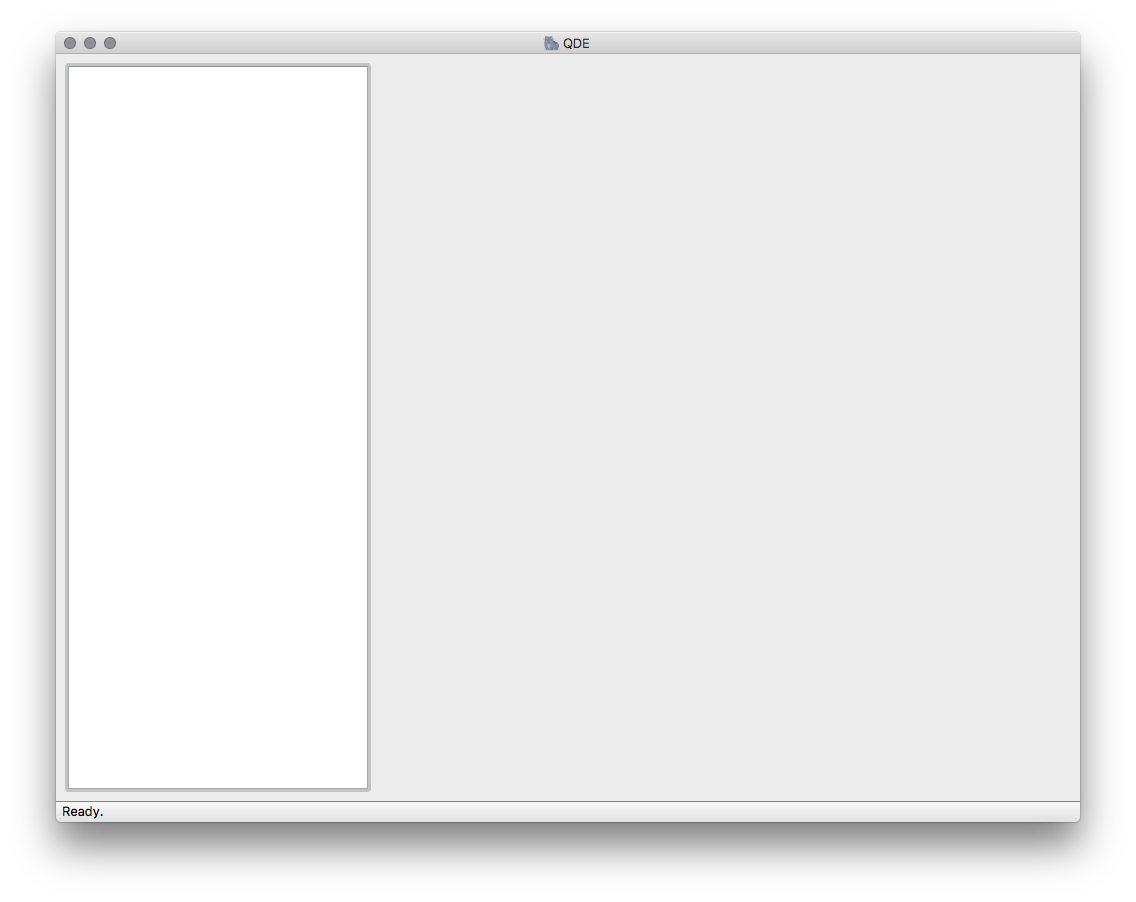
\includegraphics[width=0.5\textwidth]{./images/qde_alpha_02.png}
\caption{\label{fig:editor-alpha-02}
The QDE editor application having the scene graph widget added, which is visible as a blank, white rectangle on the left of the window.}
\end{figure}

For finally being able to manage scenes within the scene graph, a few aspects
are still missing, which will be tackled now.

First of all, the scene graph appears to hold no data at all. This is not
surprising, as no scene nodes were added by now, which might be a good point to
start with. Actually this is not the entire truth, as the root node (view model)
was already added within the scene graph controller. The controller emits the
signal, that a row was inserted, but no other component is receiving this
signal. Obviously this could be achieved by connecting the scene graph
controller and the scene graph view, but as Qt's model/view approach is at least
partially used, simply setting the view's model leads to the same result while
providing greater functionality.

\begin{listing}[H]
\begin{minted}[,fontsize=\footnotesize,linenos,bgcolor=bashcodebg]{python}
<app-application-methods-setup-connections>=
    <<app-application-methods-setup-connections-01>>
\end{minted}
\caption{\label{lst:app-application-methods-setup-connections-01}
The method \texttt{setup\_connections} being defined by setting the scene graph widget's model.}
\end{listing}

The component that ties the layers together, is, as previously described, the
main application. This means, that the main application has to provide all the
necessary data structures and controllers. Regarding the scene graph this means
setting up a root scene (as a domain-/data-model) and setting up the scene graph
controller. As the main application's layer, the \texttt{application} layer,
is directly below the layer of the view models, \texttt{gui\_domain} this
opposes no problem.

Therefore the root scene as well as the scene graph controller will be
implemented in the main application's \texttt{setup\_components} method,
whereas setting the scene graph widget's model will be implemented in the
\texttt{setup\_connections} method.

\begin{listing}[H]
\begin{minted}[,fontsize=\footnotesize,linenos,bgcolor=bashcodebg]{python}
<app-application-methods-setup-components>+=
    <<app-application-methods-setup-components-01>>
\end{minted}
\caption{The method \texttt{setup\_components} being expanded by the creation of the root scene as well as the scene graph controller.}
\end{listing}

The necessary imports are still missing however, so those are added to the main
application's imports.

\begin{listing}[H]
\begin{minted}[,fontsize=\footnotesize,linenos,bgcolor=bashcodebg]{python}
<app-application-project-imports>+=
    from qde.editor.gui import main_window as qde_main_window
    from qde.editor.domain import scene
    from qde.editor.application import scene_graph
\end{minted}
\caption{Expansion of the main application's imports by the necessary packages.}
\end{listing}

The application is still not showing the desired result: The display of the
scene graph in form of a tree containing the root node. When looking at the
outputs of the application, the messages as seen in listing \ref{lst:app-error-01} can
be observed.

\begin{listing}[H]
\begin{minted}[,fontsize=\footnotesize,linenos,bgcolor=bashcodebg]{bash}
NotImplementedError: QAbstractItemModel.columnCount() is abstract and must be overridden
NotImplementedError: QAbstractItemModel.rowCount() is abstract and must be overridden
\end{minted}
\caption{\label{lst:app-error-01}
Output (erroneous) when running the editor application.}
\end{listing}

The messages from listing \ref{lst:app-error-01} state, that not all of the necessary
methods from the sub-classed \texttt{QAbstractItemModel} are implemented yet.
Currently the methods \texttt{columnCount} and \texttt{rowCount} are
missing. Those methods return ``the number of columns for the children of the
given
parent''\footnote{\url{http://doc.qt.io/qt-5/qabstractitemmodel.html\#columnCount}}
and ``the number of rows under the given
parent''\footnote{\url{http://doc.qt.io/qt-5/qabstractitemmodel.html\#rowCount}}
respectively. The implementation of those missing methods are as follows in
listing \ref{lst:app-scenegraph-controller-methods-01}. The method
\texttt{columnCount} is trivial, as there will always be only two columns (as
defined by the header in listing \ref{lst:app-scenegraph}): The name of the scene and
the number of nodes it contains. The method \texttt{rowCount} shall return
\texttt{1} if the parent is invalid, otherwise it shall return the parent's children.

\begin{listing}[H]
\begin{minted}[,fontsize=\footnotesize,linenos,bgcolor=bashcodebg]{python}
<app-scenegraph-controller-methods>=
    def columnCount(self, parent):
        """Return the number of columns for the children of the given parent.
    
        :param parent: The index of the item in the scene graph, which the
                        column count shall be returned for.
        :type  parent: QtCore.QModelIndex
    
        :return: the number of columns for the children of the given parent.
        :rtype:  int
        """
    
        return len(self.header_data)

    def rowCount(self, parent):
        """Return the number of rows for the children of the given parent.
    
        :param parent: The index of the item in the scene graph, which the
                        row count shall be returned for.
        :type  parent: QtCore.QModelIndex
    
        :return: the number of rows for the children of the given parent.
        :rtype:  int
        """
    
        if not parent.isValid():
            return 1
    
        # Get the actual object stored by the parent. In this case it is a
        # SceneGraphViewModel.
        node = parent.internalPointer()
    
        return len(node.children())
\end{minted}
\caption{\label{lst:app-scenegraph-controller-methods-01}
The code block \texttt{<<app-scenegraph-controller-methods>>}, defining the methods \texttt{columnCount} and \texttt{rowCount} within the scene controller.}
\end{listing}

When running the application now, there is still an error message, although a
new one as can be seen in listing \ref{lst:app-error-02}.

\begin{listing}[H]
\begin{minted}[,fontsize=\footnotesize,linenos,bgcolor=bashcodebg]{bash}
NotImplementedError: QAbstractItemModel.index() is abstract and must be overridden
\end{minted}
\caption{\label{lst:app-error-02}
Output (erroneous) when running the editor application.}
\end{listing}

This time the \texttt{index} method is missing in the scene controller.
According the documentation, the method ``returns the index of the item in the
model specified by the given row, column and parent
index.''\footnote{\url{http://doc.qt.io/qt-5/qabstractitemmodel.html\#index}}
Furthermore, ``when reimplementing this function in a subclass, call
createIndex() to generate model indexes that other components can use to refer
to items in your
model.''\footnote{\url{http://doc.qt.io/qt-5/qabstractitemmodel.html\#index}}

The implementation of the missing method \texttt{index} is as follows in
listing \ref{lst:app-scenegraph-controller-methods-02}. The method needs to return the
index of the given row and column for the given parent. There are two cases
however: either the parent is valid or it is not. In the former case, the scene
graph view model of the parent is extracted and an index based on the row, the
column and the child node at the given row as parent is being created. In the
latter case, when the given parent is not valid, an index based on the scene
graph's root node is created.

\begin{listing}[H]
\begin{minted}[,fontsize=\footnotesize,linenos,bgcolor=bashcodebg]{python}
<app-scenegraph-controller-methods>+=
    def index(self, row, column, parent=QtCore.QModelIndex()):
        """Return the index of the item in the model specified by the given row,
        column and parent index.
    
        :param row: The row for which the index shall be returned.
        :type  row: int
        :param column: The column for which the index shall be returned.
        :type column: int
        :param parent: The parent index of the item in the model. An invalid model
                       index is given as the default parameter.
        :type parent: QtQore.QModelIndex
    
        :return: the model index based on the given row, column and the parent
                 index.
        :rtype: QtCore.QModelIndex
        """
    
        # If the given parent (index) is not valid, create a new index based on the
        # currently set root node
        if not parent.isValid():
            return self.createIndex(row, column, self.root_node)
    
        # The internal pointer of the the parent (index) returns a scene graph view
        # model
        parent_node = parent.internalPointer()
        child_nodes = parent_node.children()
    
        return self.createIndex(row, column, child_nodes[row])
\end{minted}
\caption{\label{lst:app-scenegraph-controller-methods-02}
The code block \texttt{<<app-scenegraph-controller-methods>>}, is expanded by the \texttt{index} method within the scene controller.}
\end{listing}

Although the scene graph is showing now two columns when running the editor
application, there are still error messages, as shown in listing \ref{lst:app-error-03}.

\begin{listing}[H]
\begin{minted}[,fontsize=\footnotesize,linenos,bgcolor=bashcodebg]{bash}
NotImplementedError: QAbstractItemModel.parent() is abstract and must be overridden
NotImplementedError: QAbstractItemModel.data() is abstract and must be overridden
\end{minted}
\caption{\label{lst:app-error-03}
Output (erroneous) when running the editor application.}
\end{listing}

The methods \texttt{parent} and \texttt{data} are missing from the
implementation. The Qt documentation states about \texttt{parent}:
``Returns the parent of the model item with the given index. If the item has no
parent, an invalid QModelIndex is returned.

A common convention used in models that expose tree data structures is that only
items in the first column have children. For that case, when reimplementing this
function in a subclass the column of the returned QModelIndex would be 0.

When reimplementing this function in a subclass, be careful to avoid calling
QModelIndex member functions, such as QModelIndex::parent(), since indexes
belonging to your model will simply call your implementation, leading to
infinite
recursion.''\footnote{\url{http://doc.qt.io/qt-5/qabstractitemmodel.html\#parent}}

Those remarks lead to the implementation, that can be seen in listing
\ref{lst:app-scenegraph-controller-methods-03}.

\begin{listing}[H]
\begin{minted}[,fontsize=\footnotesize,linenos,bgcolor=bashcodebg]{python}
<app-scenegraph-controller-methods>+=
    def parent(self, model_index):
        """Return the parent of the model item with the given index. If the item has
        no parent, an invalid QModelIndex is returned.
    
        :param model_index: The model index which the parent model index shall be
                            derived for.
        :type model_index: int
    
        :return: the model index of the parent model item for the given model index.
        :rtype: QtCore.QModelIndex
        """
    
        if not model_index.isValid():
            return QtCore.QModelIndex()
    
        # The internal pointer of the the model index returns a scene graph view
        # model.
        node = model_index.internalPointer()
        if node.parent() is None:
            return QtCore.QModelIndex()
        else:
            return self.createIndex(node.parent().row, 0, node.parent())
\end{minted}
\caption{\label{lst:app-scenegraph-controller-methods-03}
The code block \texttt{<<app-scenegraph-controller-methods>>}, is expanded by the \texttt{parent} method within the scene controller.}
\end{listing}

About the \texttt{data} method, the Qt documentation says the following:

``Returns the data stored under the given role for the item referred to by the
index.

Note: If you do not have a value to return, return an invalid QVariant instead
of returning
0.''\footnote{\url{http://doc.qt.io/qt-5/qabstractitemmodel.html\#data}}

The scene graph stores two different kinds of data: the name of the scene and its
nodes. Which of the two gets returned depends on the column. The first column,
column 0, returns the name, where as the second column, column 1, returns the
number of nodes the scene contains. It is not yet possible to implement the
second case, as scenes itself do not exist (as view models) and are not yet
provided as a reference within the scene graph view model.

For still being able to follow the current stream of thought, only a minimalist
realization of the scene view model class \texttt{SceneViewModel} is provided
by now, as can be seen in listing \ref{lst:guidomain-scene-sceneviewmodel}.

\begin{listing}[H]
\begin{minted}[,fontsize=\footnotesize,linenos,bgcolor=bashcodebg]{python}
<guidomain-scene-body>+=
    class SceneViewModel(Qt.QObject):
        """View model representing a scene.
    
        The SceneViewModel corresponds to an SceneGraphViewModel entry within the
        scene graph.
        """
    
        pass
\end{minted}
\caption{\label{lst:guidomain-scene-sceneviewmodel}
Expansion of the \texttt{scene} module, which is within the \texttt{gui\_domain} layer, by the \texttt{SceneViewModel} class. Note, that the implementation of the class provides no functionality at all at the moment.}
\end{listing}

Having the scene view model class defined, it may now be used by the scene graph
view model. This reference will then be used by the scene graph controller for
getting the number of nodes a scene contains.

\begin{listing}[H]
\begin{minted}[,fontsize=\footnotesize,linenos,bgcolor=bashcodebg]{python}
<guidomain-scene-scenegraphviewmodel-constructor>+=
        self.scene_view_model = SceneViewModel()
\end{minted}
\caption{\label{lst:guidomain-scene-scenegraphviewmodel-constructor-01}
Expansion of the constructor of the \texttt{SceneGraphViewModel} class by a reference to a scene view model.}
\end{listing}

All prerequisites for implementing the \texttt{data} method of the scene
graph controller are now met and the method may therefore now be implemented.
The method has two parameters: the model index and the role. The model index
holds the position of the item within the data model. The role indicates what
type of data is provided. Currently the only role considered is the display of
models (further information may be found
at\footnote{\url{http://doc.qt.io/qt-5/qt.html\#ItemDataRole-enum}}).
Depending on the column of the model index, either the name of the scene graph
node or the number of nodes its scene holds is returned.

\begin{listing}[H]
\begin{minted}[,fontsize=\footnotesize,linenos,bgcolor=bashcodebg]{python}
<app-scenegraph-controller-methods>+=
    def data(self, model_index, role=QtCore.Qt.DisplayRole):
        """Return the data stored unter the given role for the item referred by the
        index.
    
        :param model_index: The (data-) model index of the item.
        :type model_index: int
        :param role: The role which shall be used for representing the data. The
                     default (and currently only supported) is displaying the data.
        :type role:  QtCore.Qt.DisplayRole
    
        :return: the data stored under the given role for the item referred by the
                 given index.
        :rtype:  str
        """
    
        if not model_index.isValid():
            return None
    
        # The internal pointer of the model index returns a scene graph view
        # model.
        node = model_index.internalPointer()
    
        if role == QtCore.Qt.DisplayRole:
            # Return either the name of the scene or its number of nodes.
            column = model_index.column()
    
            if column == 0:
                return node.name
            elif column == 1:
                return node.scene_view_model.graph_node_count
\end{minted}
\caption{\label{lst:app-scenegraph-controller-methods-04}
The code block \texttt{<<app-scenegraph-controller-methods>>} is expanded by the \texttt{data} method within the scene controller.}
\end{listing}

The editor application would at this point still produce an error when being
run. The \texttt{data} method accesses a property of the scene view model
when getting the second column, the number of nodes a scene contains:
\texttt{graph\_node\_count}. As the scene view model is only a placeholder at the
moment, it is necessary to implement that property first. As the name says, the
property \texttt{graph\_node\_count} returns the number of graph nodes a scene view
model contains. Therefore the scene view model needs to hold graph nodes as a
list which leads to the definition of its constructor before implementing the
\texttt{graph\_node\_count} method.

\begin{listing}[H]
\begin{minted}[,fontsize=\footnotesize,linenos,bgcolor=bashcodebg]{python}
<guidomain-scene-sceneviewmodel-constructor>=
    def __init__(self):
        """Constructor."""
    
        self.graph_nodes = []
\end{minted}
\caption{\label{lst:guidomain-scene-scenegraphviewmodel-constructor}
Definition of the constructor of the \texttt{SceneViewModel} class.}
\end{listing}

The method \texttt{graph\_node\_count} then simply returns the length of the
graph node list, as can be seen in listing
\ref{lst:guidomain-scene-sceneviewmodel-methods-graphnodecount}.

\begin{listing}[H]
\begin{minted}[,fontsize=\footnotesize,linenos,bgcolor=bashcodebg]{python}
<guidomain-scene-sceneviewmodel-methods>+=
    @property
    def graph_node_count(self):
        """Return the number of graph nodes, that this scene contains."""
    
        return len(self.graph_nodes)
\end{minted}
\caption{\label{lst:guidomain-scene-sceneviewmodel-methods-graphnodecount}
Expansion of the scene view model's methods by adding the \texttt{graph\_node\_count} property.}
\end{listing}

When launching the editor application now, the scene graph is shown containing
the root node, as intended. One small detail is still left although. The header
data was defined in the scene graph controller, but it is not shown correctly.
Only the numbers 1 and 2 are shown as header. To get the header display the
column names correctly, the \texttt{headerData} method has to be implemented.

The Qt documentation states: ``Returns the data for the given role and section
in the header with the specified orientation.

For horizontal headers, the section number corresponds to the column number.
Similarly, for vertical headers, the section number corresponds to the row
number.''\footnote{\url{http://doc.qt.io/qt-5/qabstractitemmodel.html\#headerData}}

At the moment only the displaying-role and a horizontal orientation shall be
supported. The sections are given by the two columns 0 and 1, which correspond
to the header data. The implementation of the \texttt{headerData} is shown in
listing \ref{lst:app-scenegraph-controller-methods-header-data}.

\begin{listing}[H]
\begin{minted}[,fontsize=\footnotesize,linenos,bgcolor=bashcodebg]{python}
<app-scenegraph-controller-methods>+=
    def headerData(self, section, orientation=QtCore.Qt.Horizontal,
                   role=QtCore.Qt.DisplayRole):
        """Return the data for the given role and section in the header with the
        specified orientation.
    
        Currently vertical is the only supported orientation. The only supported
        role is DisplayRole. As the sections correspond to the header, there are
        only two supported sections: 0 and 1. If one of those parameters is not
        within the described values, None is returned.
    
        :param section: the section in the header. Currently only 0 and 1 are
                        supported.
        :type  section: int
        :param orientation: the orientation of the display. Currently only
                            Horizontal is supported.
        :type orientation:  QtCore.Qt.Orientation
        :param role: The role which shall be used for representing the data. The
                     default (and currently only supported) is displaying the data.
        :type role:  QtCore.Qt.DisplayRole
    
        :return: the header data for the given section using the given role and orientation.
        :rtype:  str
        """
    
        if (
                orientation == QtCore.Qt.Horizontal  and
                role        == QtCore.Qt.DisplayRole and
                section     in [0, 1]
        ):
            return self.header_data[section]
\end{minted}
\caption{\label{lst:app-scenegraph-controller-methods-header-data}
Expansion of the scene graph controller's methods by adding the \texttt{headerData} method which overwrites the method inherited by \texttt{QAbstractItemModel}.}
\end{listing}

\begin{figure}[H]
\centering
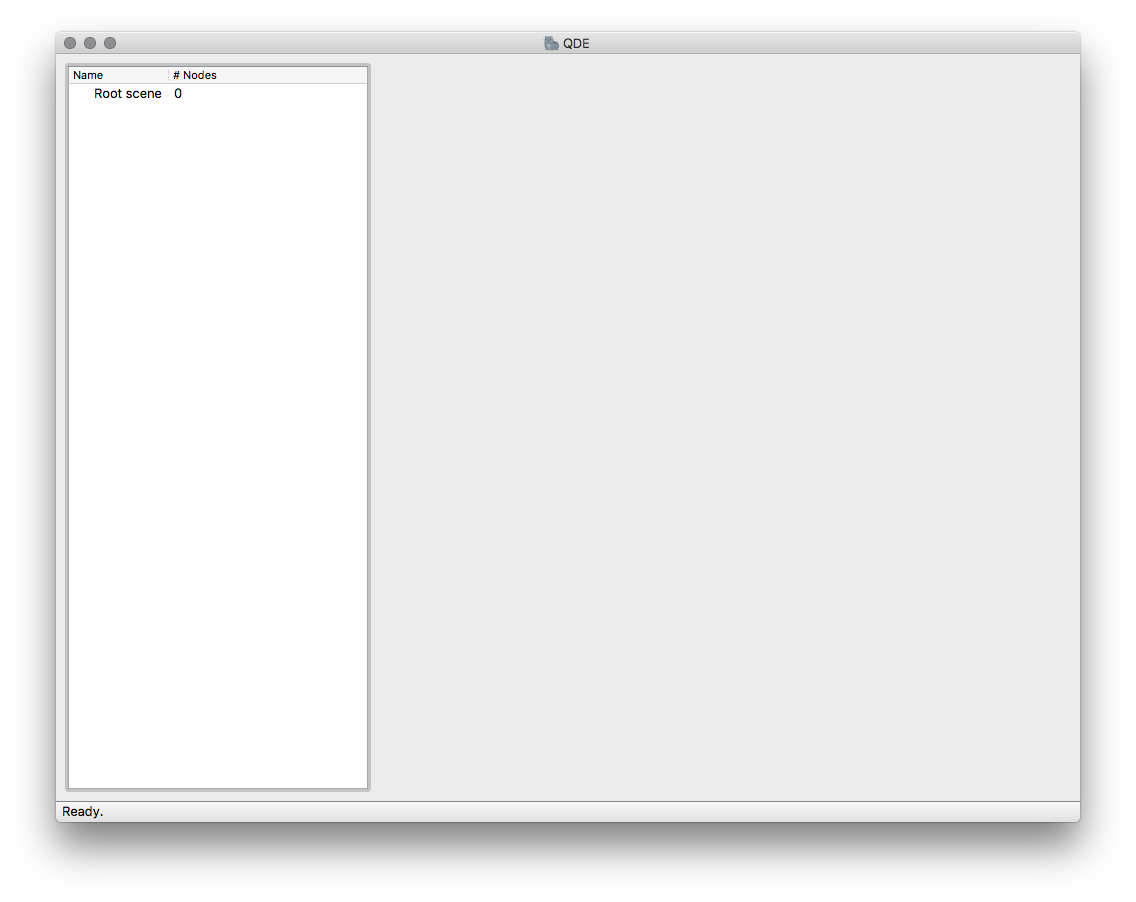
\includegraphics[width=0.5\textwidth]{./images/qde_alpha_03.png}
\caption{\label{fig:editor-alpha-03}
The QDE editor application showing the scene graph widget, containing the root node of the scene graph.}
\end{figure}

So far the application creates an instance of a scene model through the main
application, then managed by the scene graph controller. But for having only a
single (root-) scene, the whole scene graph architecture would be a massive
overkill. Instead it shall be possible to have multiple and nested scenes, what
allows the creation of diversified animations. Therefore the scene graph view
needs to provide at least the creation of new nodes, the deletion of existing
nodes and the selection of a existing nodes. First the selection of existing
nodes is implemented.

To detect if a node was selected within the scene tree of the scene graph view,
the selection model provides the \texttt{selectionChanged} signal. The
selection model is inherent in the data model of the \texttt{QTreeView}. For
being able to use the signal, the \texttt{setModel} method of the tree view
must be overridden. It is however very important to call the very same method on
the parent first. When setting the model, the root item of the model is set to be
selected.
For more flexibility, the slot \texttt{on\_tree\_item\_selected} will be
triggered upon a selection of a tree item. The implementation of those aspects
can be seen in listings \ref{lst:gui-scene-system-imports-01},
\ref{lst:gui-scene-project-imports-01}, \ref{lst:gui-scene-graph-signals-01},
\ref{lst:gui-scene-graph-methods-set-model} and \ref{lst:gui-scene-graph-slots-01}.

\begin{listing}[H]
\begin{minted}[,fontsize=\footnotesize,linenos,bgcolor=bashcodebg]{python}
<gui-scene-system-imports>=
    from PyQt5 import Qt
    from PyQt5 import QtCore
\end{minted}
\caption{\label{lst:gui-scene-system-imports-01}
Definition of the necessary system imports for selecting tree items within the view's scene package.}
\end{listing}

\begin{listing}[H]
\begin{minted}[,fontsize=\footnotesize,linenos,bgcolor=bashcodebg]{python}
<gui-scene-project-imports>=
    from qde.editor.gui_domain import scene
\end{minted}
\caption{\label{lst:gui-scene-project-imports-01}
Definition of the necessary imports for selecting tree items within the view's scene package.}
\end{listing}

\begin{listing}[H]
\begin{minted}[,fontsize=\footnotesize,linenos,bgcolor=bashcodebg]{python}
<gui-scene-graph-signals>=
    tree_item_selected = QtCore.pyqtSignal(scene.SceneViewModel)
\end{minted}
\caption{\label{lst:gui-scene-graph-signals-01}
Definition of the signal in case tree items are selected.}
\end{listing}

\begin{listing}[H]
\begin{minted}[,fontsize=\footnotesize,linenos,bgcolor=bashcodebg]{python}
<gui-scene-graph-methods>+=
    def setModel(self, model):
        """Set the model for the view to present.
    
        This method is only used for being able to use the selection model's
        selectionChanged method and setting the current selection to the root node.
    
        :param model: The item model which the view shall present.
        :type  model: QtCore.QAbstractItemModel
        """
    
        super(SceneGraphView, self).setModel(model)
    
        selection_model = self.selectionModel()
        selection_model.selectionChanged.connect(
            self.on_tree_item_selected
        )
    
        self.setCurrentIndex(model.index(0, 0))
\end{minted}
\caption{\label{lst:gui-scene-graph-methods-set-model}
The overridden \texttt{setModel} method coming from \texttt{QTreeView} being added to the methods of the scene graph view class.}
\end{listing}

\begin{listing}[H]
\begin{minted}[,fontsize=\footnotesize,linenos,bgcolor=bashcodebg]{python}
<gui-scene-graph-slots>+=
    @QtCore.pyqtSlot(QtCore.QItemSelection, QtCore.QItemSelection)
    def on_tree_item_selected(self, selected, deselected):
        """Slot which is called when the selection within the scene graph view is
        changed.
    
        The previous selection (which may be empty) is specified by the deselected
        parameter, the new selection is specified by the selected paramater.
    
        This method emits the selected scene graph item as scene graph view model.
    
        :param selected: The new selection of scenes.
        :type  selected: QtCore.QModelIndex
        :param deselected: The previous selected scenes.
        :type  deselected: QtCore.QModelIndex
        """
    
        selected_item = selected.first()
        selected_index = selected_item.indexes()[0]
        selected_scene_graph_view_model = selected_index.internalPointer()
        self.tree_item_selected.emit(selected_scene_graph_view_model)
\end{minted}
\caption{\label{lst:gui-scene-graph-slots-01}
Definition of the slot which gets called in case tree items are selected.}
\end{listing}

In the same manner the adding and removal of scenes is implemented. However, the
tree widgets does not provide direct signals for those cases as it is the case
when selecting a tree item, instead actions have to be used. Two actions are
implemented: one for adding a new item and one for removing an existing item.

An action gets triggered, typically by hovering over some item (in terms of a
context menu for example) or by pressing a defined shortcut. For the adding and
the removal the latter will be used. As the particular shortcut shall only be
valid for the widget, the \texttt{WidgetShortcut} shortcut context is used.
Adding of a scene item shall happen when pressing the \texttt{a} key on the keyboard,
removal of a selected node upon the press of the \texttt{delete} key on the keyboard.

The actions have to be added to the scene graph view and their
\texttt{triggered} signal is connected with the slot \texttt{on\_new\_tree\_item}
and \texttt{on\_tree\_item\_removed} respectively.

The implementation of the addition and removal of tree items within the scene
graph view is shown in listings \ref{lst:gui-scene-graph-slots-on-tree-item-added} and
\ref{lst:gui-scene-graph-slots-on-tree-item-added}.

Taking a step back at this point, the (main-) functionality of the editor
application is as follows. When starting, an instance of the
\texttt{Application} class is spawned. As stated before, this class
is a central aspect of the application as it connects the various layers of the
architecture. The \texttt{Application} class spawns the main window, creates
the root scene of the application and spawns the scene graph controller by
providing it with the root scene.

\begin{listing}[H]
\begin{minted}[,fontsize=\footnotesize,linenos,bgcolor=bashcodebg]{python}
<gui-scene-graph-signals>+=
    tree_item_added = QtCore.pyqtSignal(QtCore.QModelIndex)
\end{minted}
\caption{\label{lst:gui-scene-graph-signals-tree-item-removed}
The signal in case a tree item is added gets appended to the scene graph widget's signals.}
\end{listing}
\begin{listing}[H]
\begin{minted}[,fontsize=\footnotesize,linenos,bgcolor=bashcodebg]{python}
<gui-scene-graph-signals>+=
    tree_item_removed = QtCore.pyqtSignal(QtCore.QModelIndex)
\end{minted}
\caption{\label{lst:gui-scene-graph-signals-tree-item-removed}
The signal in case a tree item is removed gets appended to the scene graph widget's signals.}
\end{listing}

\begin{listing}[H]
\begin{minted}[,fontsize=\footnotesize,linenos,bgcolor=bashcodebg]{python}
<gui-scene-graph-constructor>+=
    new_action_label = QtCore.QCoreApplication.translate(
        __class__.__name__, 'New scene'
    )
    new_action = QtWidgets.QAction(new_action_label, self)
    new_action.setShortcut(Qt.QKeySequence('a'))
    new_action.setShortcutContext(QtCore.Qt.WidgetShortcut)
    new_action.triggered.connect(self.on_new_tree_item)
    self.addAction(new_action)
    
    remove_action_label = QtCore.QCoreApplication.translate(
        __class__.__name__, 'Remove selected scene(s)'
    )
    remove_action = QtWidgets.QAction(remove_action_label, self)
    remove_action.setShortcut(Qt.QKeySequence('Delete'))
    remove_action.setShortcutContext(QtCore.Qt.WidgetShortcut)
    remove_action.triggered.connect(self.on_tree_item_removed)
    self.addAction(remove_action)
\end{minted}
\caption{\label{lst:gui-scene-graph-constructor-01}
The actions to add a new scene and to remove existing scenes are added to the constructor of the scene graph view.}
\end{listing}

\begin{listing}[H]
\begin{minted}[,fontsize=\footnotesize,linenos,bgcolor=bashcodebg]{python}
<gui-scene-graph-slots>+=
    @QtCore.pyqtSlot()
    def on_new_tree_item(self):
        """Slot which is called when a new tree item was added by the scene graph
        view.
    
        This method emits the selected scene graph item as new tree item in form of
        a scene graph view model.
        """
    
        selected_indexes = self.selectedIndexes()
    
        # Sanity check: is actually an item selected?
        if len(selected_indexes) > 0:
            selected_item = selected_indexes[0]
            self.tree_item_added.emit(selected_item)
                    self.logger.debug("A new scene graph item was added.")
\end{minted}
\caption{\label{lst:gui-scene-graph-slots-on-tree-item-added}
The \texttt{on\_new\_tree\_item} slot is added to the scene graph view's slots.}
\end{listing}

\begin{listing}[H]
\begin{minted}[,fontsize=\footnotesize,linenos,bgcolor=bashcodebg]{python}
<gui-scene-graph-slots>+=
    @QtCore.pyqtSlot()
    def on_tree_item_removed(self):
        """Slot which is called when a one or multiple tree items were removed by
        the scene graph view.
    
        This method emits the removed scene graph item in form of scene graph view
        models.
        """
    
        selected_indexes = self.selectedIndexes()
    
        # Sanity check: is actually an item selected? And has that item a parent?
        # We only allow removal of items with a valid parent, as we do not want to
        # have the root item removed.
        if len(selected_indexes) > 0:
            selected_item = selected_indexes[0]
            if selected_item.parent().isValid():
                self.tree_item_removed.emit(selected_item)
                    self.logger.debug((
                        "The scene graph item at row {row} "
                        "and column {column} was removed."
                    ).format(
                        row=selected_item.row(),
                        column=selected_item.column()
                    ))
\end{minted}
\caption{\label{lst:gui-scene-graph-slots-on-tree-item-removed}
The \texttt{on\_tree\_item\_removed} slot is added to the scene graph view's slots.}
\end{listing}

When launching the editor application now, the root scene is selected within the
scene graph. When pressing the \texttt{a} or the \texttt{delete} key on the keyboard nothing
happens. But why does nothing happen? Let us reconsider.

Both times, when one of the two keys is pressed, the corresponding slot is
hopefully called. When the scene graph has a selection, one of the two signals,
\texttt{tree\_item\_added} or \texttt{tree\_item\_removed}, is emitted.
The problem seems to be, that currently no other component is paying attention
to those signals. So let us connect the two signals with a corresponding slot.
As stated before, the \texttt{Application} class acts as a connection between
layers and therefore inter-layer connections have to happen there. The
implementation of the connections is shown in listing
\ref{lst:app-application-methods-setup-connections-02}.

\begin{listing}[H]
\begin{minted}[,fontsize=\footnotesize,linenos,bgcolor=bashcodebg]{python}
<app-application-methods-setup-connections>+=
    self.main_window.scene_graph_widget.tree_item_added.connect(
        self.scene_graph_controller.on_tree_item_added
    )
    self.main_window.scene_graph_widget.tree_item_removed.connect(
        self.scene_graph_controller.on_tree_item_removed
    )
\end{minted}
\caption{\label{lst:app-application-methods-setup-connections-02}
Connections between the scene graph view and the scene graph controller are added to the \texttt{setup\_connections} method of the main application.}
\end{listing}

Setting up the connections as shown in listing
\ref{lst:app-application-methods-setup-connections-02} connects the scene graph view
with the controller. But currently the controller does not know what to do in
the case an scene graph item is added or removed as the needed slots are
missing.

But what shall actually happen upon those events? In the case a scene graph item
is added, a new scene graph entry (a row) has to be added to the data model. In
the case an existing scene graph item is being removed, the item has to be
removed from the data model.

As the scene graph controller inherits from \texttt{QAbstractItemModel} the
corresponding methods, \texttt{insertRows} and \texttt{removeRows}, have
to be implemented. First, let us implement the slots as they are very easy to
implement. Implementing \texttt{on\_tree\_item\_added} is straightforward: the
\texttt{insertRows} method is called by providing the row, the count and
the parent of the new item. Note, that the row is currently always zero. The
implementation can be seen in listing
\ref{lst:app-scenegraph-controller-slots-01}.

\begin{listing}[H]
\begin{minted}[,fontsize=\footnotesize,linenos,bgcolor=bashcodebg]{python}
<app-scenegraph-controller-slots>+=
    @QtCore.pyqtSlot(QtCore.QModelIndex)
    def on_tree_item_added(self, parent_index):
        """Add a new row under the given parent.
    
        :param parent_index: The index of the parent item.
        :type  parent_index: QtCore.QModelIndex
        """
    
        if parent_index.isValid():
            self.insertRows(0, 1, parent_index)
        else:
            # TODO: Log warning or error
            pass
\end{minted}
\caption{\label{lst:app-scenegraph-controller-slots-01}
The slot \texttt{on\_tree\_item\_added} is being added to the scene graph controller's slots.}
\end{listing}

The implementation of \texttt{on\_tree\_item\_added} is analogous: the
\texttt{removeRows} method is called by providing the row, the count and
the parent of the new item. The implementation can be seen in listing
\ref{lst:app-scenegraph-controller-slots-02}.

\begin{listing}[H]
\begin{minted}[,fontsize=\footnotesize,linenos,bgcolor=bashcodebg]{python}
<app-scenegraph-controller-slots>+=
    @QtCore.pyqtSlot(QtCore.QModelIndex)
    def on_tree_item_removed(self, selected_index):
        """Remove the currently selected item from the scene graph.
    
        :param selected_index: The index of the current selection.
        :type  selected_index: QtCore.QModelIndex
        """
    
        if selected_index.isValid():
            row    = selected_index.row()
            parent = selected_index.parent()
            self.removeRows(row, 1, parent)
        else:
            # TODO: Log warning or error
            pass
\end{minted}
\caption{\label{lst:app-scenegraph-controller-slots-02}
The slot \texttt{on\_tree\_item\_removed} is being added to the scene graph controller's slots.}
\end{listing}

Having the slots for adding and removing scene graph items implemented, the
actual methods for these actions are still missing. So, let us implement these
now.

When inserting a row, the first thing to do is calling
\texttt{beginInsertRows} by providing the index of the parent item, the
current row and the last row of insertion (which is the current row plus the
count minus one). Then a scene model, representing the actual data structure of
a scene, as well as a scene graph view model is being created, representing the
very same scene model within the graphical user interface. The transaction is
then being ended by calling \texttt{endInsertRows}. Finally the view widget
is being told to redraw itself by emitting the \texttt{layoutChanged} signal
and the \texttt{scene\_added} signal is emitting the newly created domain
model to inform other components (subscribers) about the creation. This can be
seen in listing \ref{lst:app-scenegraph-controller-methods-insert-rows}.

\begin{listing}[H]
\begin{minted}[,fontsize=\footnotesize,linenos,bgcolor=bashcodebg]{python}
<app-scenegraph-controller-methods>+=
    def insertRows(self, row, count, parent_index=QtCore.QModelIndex()):
        """ Insert the given number of rows into the scene graph below the given
        parent.
    
        :param row: The row after which the new rows shall be inserted.
        :type  row: int
        :param count: The number of rows to insert.
        :type  count: int
        :param parent_index: The index of the parent item, under which the rows will
                             be inserted.
        :type parent_index:  QtCore.QModelIndex
    
        :return: a boolean value. True when the insertion was successful, False otherwise.
        :rtype:  bool
        """
    
        if parent_index.isValid():
            self.beginInsertRows(parent_index, row, row + count - 1)
    
            # The internal pointer of the parent index returns a scene graph view
            # model.
            parent_node = parent_index.internalPointer()
    
            domain_scene_model = domain_scene.SceneModel()
            guidomain_scene.SceneGraphViewModel(
                row=row,
                domain_object=domain_scene_model,
                parent=parent_node
            )
    
            self.endInsertRows()
    
            self.layoutChanged.emit()
            self.scene_added.emit(domain_scene_model)
        else:
            return False
\end{minted}
\caption{\label{lst:app-scenegraph-controller-methods-insert-rows}
The method \texttt{insertRows} is being added to the scene graph controller's methods.}
\end{listing}

Removing a row is very similar. Analogous, the first thing to do is calling
\texttt{beginRemoveRows} by providing the index of the parent item, the
current row and the last row of insertion (which is the current row plus the
count minus one).
The actual removal of the node is then done by getting that node from its parent
by using the provided row and the parent's column. The node is then removed by
setting its parent to \texttt{None}. Qt's data model will therefore then remove the
node. The transaction is then being ended by calling \texttt{endRemoveRows}.
Finally, again the view widget is being told to redraw itself by emitting the
\texttt{layoutChanged} signal and the \texttt{scene\_removed} signal is
emitting the linked domain model to inform other components (subscribers) about
the removal. This can be seen in listing
\ref{lst:app-scenegraph-controller-methods-remove-rows}.

\begin{listing}[H]
\begin{minted}[,fontsize=\footnotesize,linenos,bgcolor=bashcodebg]{python}
<app-scenegraph-controller-methods>+=
    def removeRows(self, row, count, parent_index=QtCore.QModelIndex()):
        """Remove the given number of rows, lying below the given parent, from the
        scene graph.
    
        :param row: The row which marks the beginning of the removal.
        :type  row: int
        :param count: The number of rows to remove starting from the given row.
        :type  count: int
        :param parent_index: The index of the parent item, under which the rows will
                             be removed.
        :type parent_index:  QtCore.QModelIndex
    
        :return: a boolean value. True when the removal was successful, False otherwise.
        :rtype:  bool
        """
    
        if parent_index.isValid():
            self.beginRemoveRows(parent_index, row, row + count - 1)
    
            node_index = parent_index.child(row, parent_index.column())
            # The internal pointer of the node index returns a scene graph view
            # model.
            node = node_index.internalPointer()
            node.setParent(None)
    
            self.endRemoveRows()
    
            self.layoutChanged.emit()
            self.scene_removed.emit(node.domain_object)
        else:
            return False
\end{minted}
\caption{\label{lst:app-scenegraph-controller-methods-remove-rows}
The method \texttt{removeRows} is being added to the scene graph controller's methods.}
\end{listing}

The newly added functionality now allows the adding and removal of scenes within
the scene graph, which can be seen in figure \ref{fig:editor-alpha-04}. The scenes are
added to (or removed from respectively) the graphical user interface as well as
the data structure.

\begin{figure}[H]
\centering
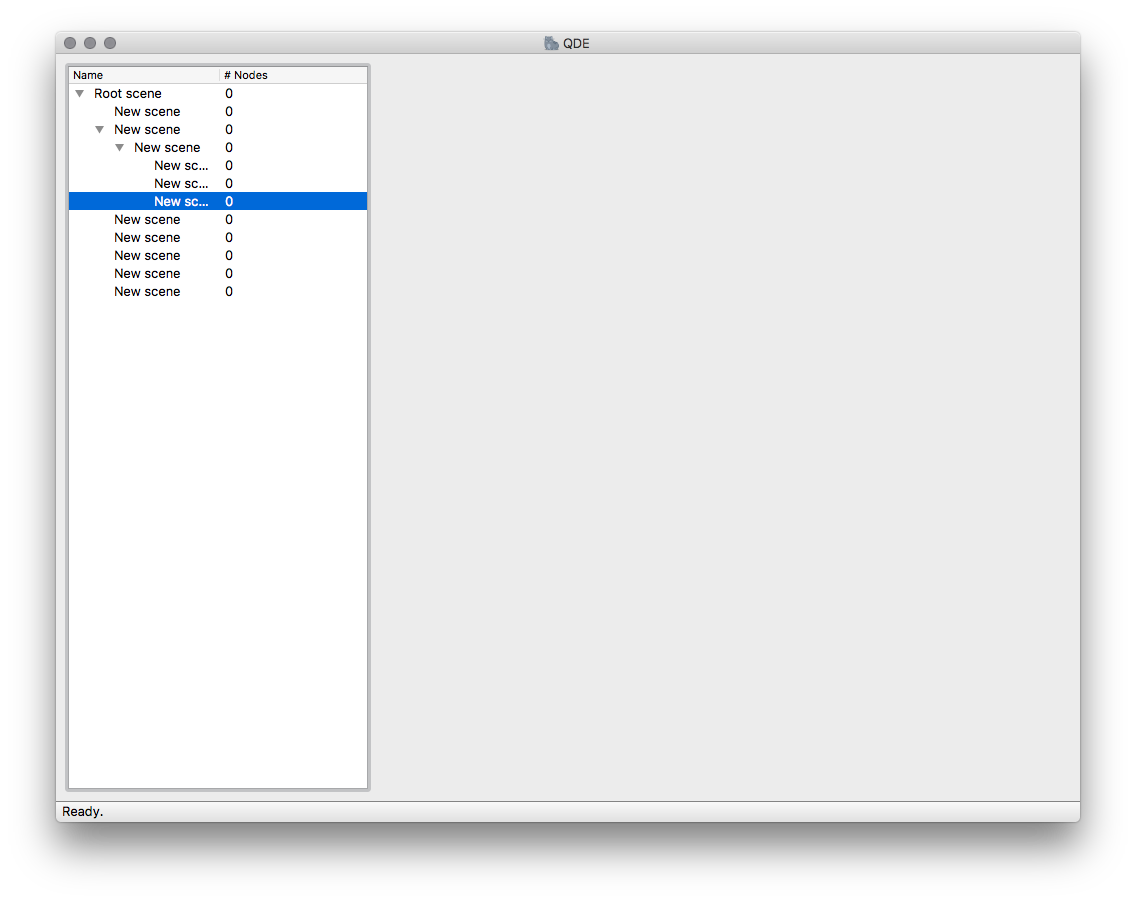
\includegraphics[width=0.5\textwidth]{./images/qde_alpha_05.png}
\caption{\label{fig:editor-alpha-04}
The QDE editor application showing the scene graph widget, containing multiple scenes.}
\end{figure}


So far the application (or rather the scene graph) seems to be working as
intended. But how do we ensure, that it really does? Without a doubt, unit and
integration tests are one of the best instruments to ensure functionality of
code. As stated before, in section \ref{sec:org5f2f7a9}, it was an intention of
this project to develop the application test driven. Due to required amount of
work for developing test driven, it was abstained from this intention and
regular unit tests are written instead, which can be found in appendix \ref{sec:org6048ce6}.

But nevertheless, it would be very handy to have at least some idea what the
code is doing at certain places and at certain times.
One of the simplest approaches to achieve this, is a verbose output at various
places of the application, which may be as simple as using Python's
\texttt{print} function. Using the \texttt{print} function may allow
printing something immediately, but it lacks of flexibility and demands each
time a bit of effort to format the output accordingly (e.g. adding the class and
the function name and so on). Python's logging facility provides much more
functionality while being able to keep things simple as well --- if needed.
The usage of the logging facility to log messages throughout the application may
later even be used to implement a widget which outputs those messages. So
logging using Python's logging facility will be implemented and applied for
being able to have feedback when needed.
\subsection{{\bfseries\sffamily DONE} Logging}
\label{sec:orge818cb4}
As logging is a very central and basic functionality, the module is placed in
the \texttt{foundation} layer.

Logging shall be provided on a class-basis, meaning that each class (which wants
to log something) needs to instantiate a logger and use a corresponding handler.

Python's logging module uses the basic configuration by default, calling the
\texttt{basicConfig} whenever something is logged for the first time. This
creates a stream handler with a basic formatter. However, the logging facility
may extensively be
configured\footnote{\url{https://docs.python.org/3/library/logging.html}}.

For example, the logging may be configured by using the ``Configuration API'',
which offers configuring the logging facility by using a dictionary. A
dictionary may very easily be created by using a JSON file.

As mentioned before, logging is a central aspect of the application. Therefore
it is the task of the main application to set up the logging facility which may
then be used by other classes through a decorator.

The main application shall therefore set up the logging facility as follows:

\begin{itemize}
\item Use either an external logging configuration or the default logging configuration.

\item When using an external logging configuration

\begin{itemize}
\item The location of the external logging configuration may be set by the
environment variable \texttt{QDE\_LOG\_CFG}.

\item Is no such environment variable set, the configuration file is assumed to be
named \texttt{logging.json} and to reside in the application's main
directory.
\end{itemize}

\item When using no external logging configuration, the default logging configuration
defined by \texttt{basicConfig} is used.

\begin{itemize}
\item Always set a level when using no external logging configuration, the default
being \texttt{INFO}.
\end{itemize}
\end{itemize}

This leads to two parameters when setting up the logging configuration: The
default path of the external logging configuration and the default logging
level when using no external logging configuration. The implementation of
setting up the logging facility can be seen in listing
\ref{lst:app-application-methods-setup-logging}.

\begin{listing}[H]
\begin{minted}[,fontsize=\footnotesize,linenos,bgcolor=bashcodebg]{python}
    <app-application-methods>+=
           def setup_logging(self,
                             default_path='logging.json',
                             default_level=logging.INFO):
               """Setup logging configuration"""
           
               env_key  = 'QDE_LOG_CFG'
               env_path = os.getenv(env_key, None)
               path     = env_path or default_path
           
               if os.path.exists(path):
                   with open(path, 'rt') as f:
                       config = json.load(f)
                       logging.config.dictConfig(config)
               else:
                   logging.basicConfig(level=default_level)
\end{minted}
\caption{\label{lst:app-application-methods-setup-logging}
The \texttt{setup\_logging} method is being added to the main application class \texttt{Application}.}
\end{listing}

\begin{listing}[H]
\begin{minted}[,fontsize=\footnotesize,linenos,bgcolor=bashcodebg]{python}
    <app-application-constructor>+=
               self.setup_logging()
\end{minted}
\caption{\label{lst:app-application-constructor-call-setup-logging}
The call of the \texttt{setup\_logging} method is being added to the main application's constructor.}
\end{listing}

\begin{listing}[H]
\begin{minted}[,fontsize=\footnotesize,linenos,bgcolor=bashcodebg]{python}
    <app-application-system-imports>+=
            import logging
            import logging.config
            import os
            import json
\end{minted}
\caption{\label{lst:app-application-system-imports-logging}
The \texttt{logging} module is added to the application module's system imports.}
\end{listing}

For not having only basic logging available, a logging configuration is defined
and provided by listing \ref{lst:logging-configuration}. The logging configuration
provides three handlers: a console handler, which logs debug messages to STDOUT,
a info file handler, which logs informational messages to a file named
\texttt{info.log}, and a error file handler, which logs errors to a file
named \texttt{error.log}. The default level is set to debug and all handlers
are used.

\begin{listing}[H]
\begin{minted}[,fontsize=\footnotesize,linenos,bgcolor=bashcodebg]{json}
    {
        "version": 1,
        "disable_existing_loggers": false,
        "formatters": {
            "simple": {
                "format": "%(asctime)s - %(levelname)-7s - %(name)s.%(funcName)s::%(lineno)s: %(message)s"
            }
        },
    
        "handlers": {
            "console": {
                "class": "logging.StreamHandler",
                "level": "DEBUG",
                "formatter": "simple",
                "stream": "ext://sys.stdout"
            },
    
            "info_file_handler": {
                "class": "logging.handlers.RotatingFileHandler",
                "level": "INFO",
                "formatter": "simple",
                "filename": "info.log",
                "maxBytes": 10485760,
                "backupCount": 20,
                "encoding": "utf8"
            },
    
            "error_file_handler": {
                "class": "logging.handlers.RotatingFileHandler",
                "level": "ERROR",
                "formatter": "simple",
                "filename": "errors.log",
                "maxBytes": 10485760,
                "backupCount": 20,
                "encoding": "utf8"
            }
        },
    
        "root": {
            "level": "DEBUG",
            "handlers": ["console", "info_file_handler", "error_file_handler"],
            "propagate": "no"
        }
    }
\end{minted}
\caption{\label{lst:logging-configuration}
The configuration of the logging facility in JSON format.}
\end{listing}

The logging configuration as shown in listing \ref{lst:logging-configuration} allows
to get an arbitrarily named logger which uses that configuration.

As stated before, logging shall be provided on a class basis. This has the
consequence, that each class has to instantiate a logging instance. To prevent
the repetition of the same code fragment over and over, Python's decorator
pattern is used\footnote{\url{https://www.python.org/dev/peps/pep-0318/}}.

The decorator will be implemented as a method named \texttt{with\_logger} in
the \texttt{common} module. All, that this method does is to set the logger
name to the name of the module it is in combined with his own name. It then
attaches a property named \texttt{logger} to the class that calls the method.
The method has therefore the following functionality.

\begin{itemize}
\item Provide a name based on the current module and class.
\begin{listing}[H]
\begin{minted}[,fontsize=\footnotesize,linenos,bgcolor=bashcodebg]{python}
    logger_name = "{module_name}.{class_name}".format(
        module_name=cls.__module__,
        class_name=cls.__name__
    )
\end{minted}
\caption{\label{logger-name}
Setting of the name based on the current module and class name.}
\end{listing}
\item Provide an easy to use interface for logging.
\begin{listing}[H]
\begin{minted}[,fontsize=\footnotesize,linenos,bgcolor=bashcodebg]{python}
    cls.logger = logging.getLogger(logger_name)
    
    return cls
\end{minted}
\caption{\label{logger-return-logger}
The logger is being attached to the class itself.}
\end{listing}
\end{itemize}

This definition of the functionality allows the actual implementation of the
logging facility which follows in listing \ref{lst:foundation-common}.

\begin{listing}[H]
\begin{minted}[,fontsize=\footnotesize,linenos,bgcolor=bashcodebg]{python}
    # -*- coding: utf-8 -*-
    
    """Module holding common helper methods."""
    
    # System imports
    import logging
    
    
    # Project imports
    
    
    
    def with_logger(cls):
        """Add a logger instance (using a stream handler) to the given class.
    
        :param cls: the class which the logger shall be added to.
        :type  cls: a class of type cls.
    
        :return: the class with the logger instance added.
        :rtype:  a class of type cls.
        """
    
            logger_name = "{module_name}.{class_name}".format(
                module_name=cls.__module__,
                class_name=cls.__name__
            )
            cls.logger = logging.getLogger(logger_name)
            
            return cls
\end{minted}
\caption{\label{lst:foundation-common}
Implementation of the logging facility as a method inside the \texttt{common}  module.}
\end{listing}

The implementation of the \texttt{with\_logger} method allows the usage of the
logging facility as a decorator as shown in the example in listing
\ref{lst:with-logger-example}.

\begin{listing}[H]
\begin{minted}[,fontsize=\footnotesize,linenos,bgcolor=bashcodebg]{python}
    # Project imports
    from qde.editor.foundation import common
    
    @common.with_logger
    def SomeClass(object):
        """This class provides literally nothing and is used only to demonstrate the
        usage of the logging decorator."""
    
        def some_method():
            """This method does literally nothing and is used only to demonstrate the
            usage of the logging decorator."""
    
            self.logger.debug(("I am some logging entry used for"
                               "demonstration purposes only."))
\end{minted}
\caption{\label{lst:with-logger-example}
The class \texttt{SomeClass} gets annotated by the \texttt{with\_logger} decorator from the \texttt{common} module. The whole class is then able to use the \texttt{logger} property as can be seen in method \texttt{some\_method}.}
\end{listing}

This brings us back to original intention: log whenever a scene is added or
removed in the scene graph view. To implement the logging three steps are
necessary. First, the \texttt{common} module needs to be imported.

\begin{listing}[H]
\begin{minted}[,fontsize=\footnotesize,linenos,bgcolor=bashcodebg]{python}
    <gui-scene-project-imports>+=
            from qde.editor.foundation import common
\end{minted}
\caption{\label{lst:gui-scene-project-imports-02}
The \texttt{common} module is added to the project imports of the \texttt{scene} module residing in the \texttt{gui} layer.}
\end{listing}

Second, the class needs the \texttt{with\_logger} decorator.

\begin{listing}[H]
\begin{minted}[,fontsize=\footnotesize,linenos,bgcolor=bashcodebg]{python}
    <gui-scene-graph-class-decorators>+=
            @common.with_logger
\end{minted}
\caption{\label{lst:gui-scene-graph-class-decorators-01}
The \texttt{with\_logger} decorator is added to the scene graph view class's decorators, <\ref{fig:gui-scene-graph}>.}
\end{listing}

And third, the actual logging needs to be added to the corresponding methods.

\begin{listing}[H]
\begin{minted}[,fontsize=\footnotesize,linenos,bgcolor=bashcodebg]{python}
    <gui-scene-graph-slots-on-tree-item-added>+=
            self.logger.debug("A new scene graph item was added.")
\end{minted}
\caption{\label{lst:gui-scene-graph-slots-on-tree-item-added-logging}
A debug message is being logged, whenever a new scene is added to the scene graph within the scene graph view.}
\end{listing}

\begin{listing}[H]
\begin{minted}[,fontsize=\footnotesize,linenos,bgcolor=bashcodebg]{python}
    <gui-scene-graph-slots-on-tree-item-removed>+=
            self.logger.debug((
                "The scene graph item at row {row} "
                "and column {column} was removed."
            ).format(
                row=selected_item.row(),
                column=selected_item.column()
            ))
\end{minted}
\caption{\label{lst:gui-scene-graph-slots-on-tree-item-removed-logging}
A debug message is being logged, whenever an existing scene is removed from the scene graph within the scene graph view.}
\end{listing}

Whenever the \texttt{a} or the \texttt{delete} key is being pressed now, when the scene graph
view is focused, the corresponding log messages appear in the standard output,
hence the console. This behavior can be seen in figure \ref{fig:editor-alpha-04}.

\begin{figure}[H]
\centering
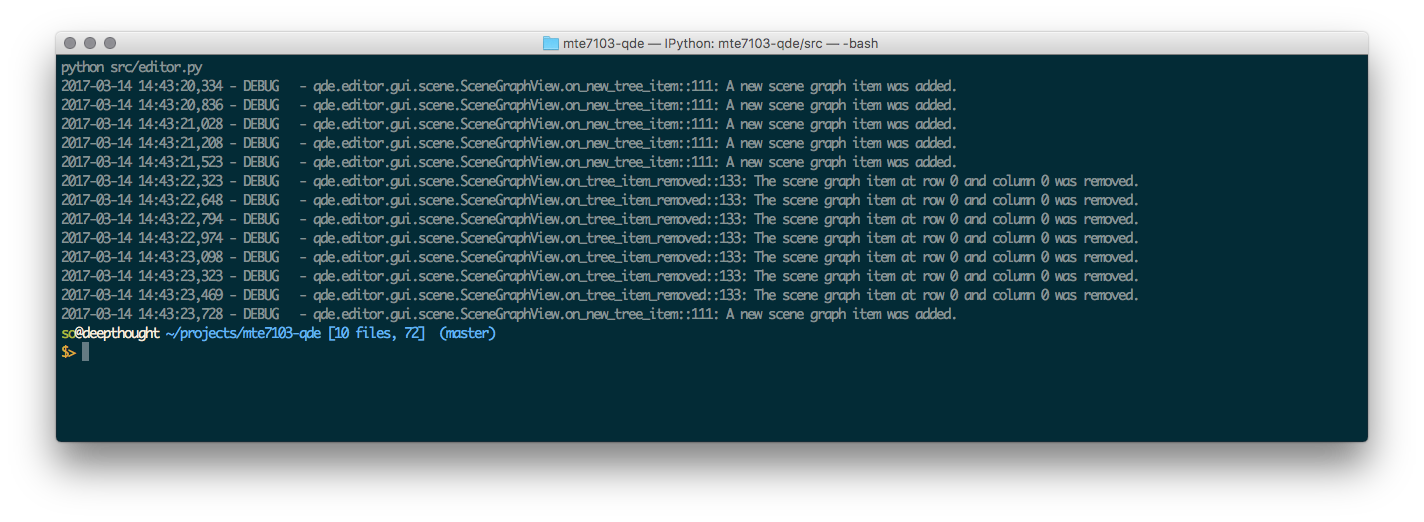
\includegraphics[width=0.5\textwidth]{./images/qde_alpha_04.png}
\caption{\label{fig:editor-alpha-04}
The console output when the \texttt{a} and the \texttt{delete} keys are pressed multiple times with the scene graph view being the active widget.}
\end{figure}

Now, having the scene graph component as well as an interface to log messages
throughout the application implemented, the next component may be approached. A
very interesting aspect to face would be the rendering. But for being able to
render something, there actually needs to exist something to render: nodes.
Nodes are being represented within the node graph. So this is a good point to
begin with the implementation of the node graph.
\subsection{{\bfseries\sffamily TODO} Node graph}
\label{sec:org8f3d3a2}
\chapter{Work log}
\label{sec:orgb2cb4f2}
\begin{description}
\item[{\textit{<2017-02-20 Mon>}}] Set up and structure the document initially.

\item[{\textit{<2017-02-21 Tue>}}] Re-structure the document, add first contents of the
implementation. Add first tries to tangle the code.

\item[{\textit{<2017-02-22 Wed>}}] Provide further content concerning the implementation:
Introduce name-spaces/initializers, first steps for a logging facility.

\item[{\textit{<2017-02-23 Thu>}}] Extend logging facility, provide (unit-) tests.
Restructure the documentation.

\item[{\textit{<2017-02-24 Fri>}}] Adapt document to output \LaTeX{} code as desired, change
styling. Begin development of the applications' main routine.

\item[{\textit{<2017-02-27 Mon>}}] Remove (unit-) tests from main document and put them into
appendix instead. Begin explaining literate programming.

\item[{\textit{<2017-02-28 Tue>}}] Provide a first draft for objectives and limitations.
Re-structure the document. Correct \LaTeX{} output.

\item[{\textit{<2017-03-01 Wed>}}] Remove split files, re-add everything to index, add
objectives.

\item[{\textit{<2017-03-02 Thu>}}] Set up project schedule. Tangle everything instead of
doing things manually. Begin changing language to English instead of German.
Re-add make targets for cleaning and building the source code.

\item[{\textit{<2017-03-03 Fri>}}] Keep work log up to date. Revise and finish chapter about
name-spaces and the project structure for now.

\item[{\textit{<2017-03-04 Sat>}}] Finish translating all already written texts from German
to English. Describe the main entry point of the application as well as the
main application itself.

\item[{\textit{<2017-03-05 Sun>}}] Finish chapter about the main entry point and the main
application for now, start describing the main window and implement its
functionality. Keep the work log up to date. Fiddle with references and
\LaTeX{} export. Find a bug: main\_window needs to be attached to a class, by
using the \texttt{self} keyword, otherwise the window does not get shown.
Introduce new make targets: one to clean Python cache files (*.pyc) and one
to run the editor application directly.

\item[{\textit{<2017-03-06 Mon>}}] Update the work log. Add an image of the editor as well as
the project schedule. Add the implementation of the main window's layout.
Implement the scene domain model. Move keyPressEvent to its own source
block instead of expanding the methods of the main window directly. Add a
section about (the architecture's) layers to the principles section. Add
Dr. Eric Dubuis as an expert to the involved persons. Introduce the 'verb'
macro for having nicer verbatim blocks. Use the given image-width for
inline images in org-mode when available.

\item[{\textit{<2017-03-07 Tue>}}] Expand the layering principles by adding a section about
the model-view-controller pattern and introduce view models. Explain and
implement the data- and the view model for scene graph items.

\item[{\textit{<2017-03-08 Wed>}}] Implement the controller for handling the scene graph.
Allow the semi-automatic creation of an API documentation by introducing
Sphinx. Introduce new make targets for creating the API documentation as
RST and as HTML.

\item[{\textit{<2017-03-10 Fri>}}] Implement the scene graph view as widget and integrate it
into the application. Update the work log. Fix typing errors. Start to
implement missing methods in the scene graph controller for being able to
use the scene graph widget.

\item[{\textit{<2017-03-13 Mon>}}] Implement the scene view model. Initialize such a model
within the scene graph view model. Implement the \texttt{headerData} as well as
the \texttt{data} methods of the scene graph controller. Update the work log. Add
an image of the editor's current state. Continue implementation of the
scene graph view model.

\item[{\textit{<2017-03-14 Tue>}}] Continue the implementation of the scene graph view model.
Implement logging. Implement logging. Implement logging. Implement logging
functionality. Log whenever a node is added or removed from the scene graph
view.

\item[{\textit{<2017-03-15 Wed>}}] Move logging further down in structure. Add connections
between scene graph view and controller. Finish implementing the adding and
removal of scene graph items. Update the work log.

Next steps: (Re-) Introduce logging. Begin implementing the node graph.

\item[{\textit{<2017-03-16 Thu>}}] Run sphinx apidoc when creating the HTML documentation.
Add an illustration about the state of the editor after finishing the
implementation of the scene graph. Change width of the images to be 50\% of
the text width. Name slots of the scene graph view explicitly to maintain
sanity. Re-add logging chapter with a corresponding introduction. Fix display
of code listings. Keep work log up to date. Add missing TODO annotations to
headings.

Next steps: Continue implementing the node graph.

\item[{\textit{<2017-03-17 Fri>}}] Change verbatim output to be less intrusive, update to do
tags, begin adding references do code fragment definitions, begin implement
the node graph. Move chapters into separate org files.
\end{description}
\chapter{{\bfseries\sffamily TODO} Bibliography}
\label{sec:org20d33d4}
\printbibliography{}
\chapter{{\bfseries\sffamily TODO} Appendix}
\label{sec:org065d257}
\section{Test cases}
\label{sec:org6048ce6}
\subsection{Test cases}
\label{sec:org6d0449e}

Zunächst wird jedoch der entsprechende Unit-Test definiert. Dieser instanziert
die Klasse und stellt sicher, dass sie ordnungsgemäss gestartet werden kann.

Als erster Schritt wird der Header des Test-Modules definiert.

\begin{listing}[H]
\begin{minted}[,fontsize=\footnotesize,linenos,bgcolor=bashcodebg]{python}
# -*- coding: utf-8 -*-

"""Module for testing QDE class."""
\end{minted}
\caption{\label{test-app-header}
Header des Test-Modules, \texttt{<<test-app-header>>}.}
\end{listing}

Dann werden die benötigen Module importiert. Es sind dies das System-Modul
\emph{sys} und das Modul \emph{application}, bei welchem es sich um die Applikation
selbst handelt. Das System-Modul \emph{sys} wird benötigt um der Applikation ggf.
Start-Argumente mitzugeben, also zum Beispiel:

\begin{listing}[H]
\begin{minted}[,fontsize=\footnotesize,linenos,bgcolor=bashcodebg]{bash}
python main.py argument1 argument2
\end{minted}
\caption{\label{fig:impl-python-call-arguments}
Aufruf des Main-Modules mit zwei Argumenten, \texttt{argument1} und \texttt{argument2}.}
\end{listing}

Der Einfachheit halber werden die Importe in zwei Kategorien unterteilt: Importe
von Pyhton-eigenen Modulen und Importe von selbst verfassten Modulen.

\begin{listing}[H]
\begin{minted}[,fontsize=\footnotesize,linenos,bgcolor=bashcodebg]{python}
# System imports
<<test-app-system-imports>>

# Project imports
<<test-app-project-imports>>
\end{minted}
\caption{\label{test-app-imports}
Definition der Importe für das Modul zum Testen der Applikation.}
\end{listing}

\begin{listing}[H]
\begin{minted}[,fontsize=\footnotesize,linenos,bgcolor=bashcodebg]{python}
# System imports
import sys
\end{minted}
\caption{Importe von Python-eigenen Modulen im Modul zum Testen der Applikation.}
\end{listing}

\begin{listing}[H]
\begin{minted}[,fontsize=\footnotesize,linenos,bgcolor=bashcodebg]{python}
# Project imports
from qde.editor.application import application
\end{minted}
\caption{\label{test-app-project-imports}
Importe von selbst verfassten Modulen im Modul zum Testen der Applikation.}
\end{listing}

Somit kann schliesslich getestet werden, ob die Applikation startet, indem diese
instanziert wird und die gesetzten Namen geprüft werden.

\begin{listing}[H]
\begin{minted}[,fontsize=\footnotesize,linenos,bgcolor=bashcodebg]{python}
def test_constructor():
    """Test if the QDE application is starting up properly."""
    app = application.QDE(sys.argv)
    assert app.applicationName() == "QDE"
    assert app.applicationDisplayName() == "QDE"
\end{minted}
\caption{\label{test-app-test-constructor}
Methode zum Testen des Konstruktors der Applikation.}
\end{listing}

Finally, one can merge the above defined elements to an executable test-module,
containing the header, the imports and the test cases (which is in this case
only a test case for testing the constructor).

\begin{listing}[H]
\begin{minted}[,fontsize=\footnotesize,linenos,bgcolor=bashcodebg]{python}
<<test-app-header>>

<<test-app-imports>>

<<test-app-test-constructor>>
\end{minted}
\caption{Modul zum Testen der Applikation.}
\end{listing}

Führt man die Testfälle nun aus, schlagen diese erwartungsgemäss fehl, da die
Klasse, und somit die Applikation, als solche noch nicht existiert. Zum jetzigen
Zeitpunkt kann noch nicht einmal das Modul importiert werden, da diese noch
nicht existiert.

\begin{listing}[H]
\begin{minted}[,fontsize=\footnotesize,linenos,bgcolor=bashcodebg]{bash}
python -m pytest qde/editor/application/test_application.py
\end{minted}
\caption{Aufruf zum Testen des Applkations-Modules.}
\end{listing}

Um sicherzustellen, dass die Protokollierung wie gewünscht funktioniert, wird
diese durch die entsprechenden Testfälle abgedeckt.

Der einfachste Testfall ist die Standardkonfiguration, also ein Aufruf ohne
Parameter.

\begin{listing}[H]
\begin{minted}[,fontsize=\footnotesize,linenos,bgcolor=bashcodebg]{python}
def test_setup_logging_without_arguments():
    """Test logging of QDE application without arguments."""
    app = application.QDE(sys.argv)
    root_logger = logging.root
    handlers = root_logger.handlers
    assert len(handlers) == 1
    handler = handlers[0]
\end{minted}
\caption{\label{test-app-test-logging-default}
Testfall 1 der Protkollierung der Hauptapplikation: Aufruf ohne Argumente.}
\end{listing}

Da obige Testfälle das \emph{logging}-Module benötigen, muss das Importieren der Module
entsprechend erweitert werden.

\begin{listing}[H]
\begin{minted}[,fontsize=\footnotesize,linenos,bgcolor=bashcodebg]{python}
import logging
\end{minted}
\caption{\label{test-app-system-imports}
Erweiterung des Importes von System-Modulen im Modul zum Testen der Applikation.}
\end{listing}

Und der Testfall muss den Testfällen hinzugefügt werden.

\begin{listing}[H]
\begin{minted}[,fontsize=\footnotesize,linenos,bgcolor=bashcodebg]{python}
<<test-app-test-logging-default>>
\end{minted}
\caption{\label{test-app-test-cases}
Hinzufügen des Testfalles 1 zu den bestehenden Testfällen im Modul zum Testen der Applikation.}
\end{listing}

Auch hierfür werden wiederum zuerst die Testfälle verfasst.

\begin{listing}[H]
\begin{minted}[,fontsize=\footnotesize,linenos,bgcolor=bashcodebg]{python}
# -*- coding: utf-8 -*-

"""Module for testing common methods class."""

# System imports
import logging

# Project imports
from qde.editor.foundation import common


@common.with_logger
class FooClass(object):
    """Dummy class for testing the logging decorator."""

    def __init__(self):
        """Constructor."""
        pass

def test_with_logger():
    """Test if the @with_logger decorator works correctly."""

    foo_instance = FooClass()
    logger = foo_instance.logger
    name = "qde.editor.foundation.test_common.FooClass"
    assert logger is not None
    assert len(logger.handlers) == 1
    handler = logger.handlers[0]
    assert type(handler) == logging.StreamHandler
    assert logger.propagate == False
    assert logger.name == name
\end{minted}
\caption{\label{fig:editor-common-logging-test}
Testfälle der Hilfsmethode zur Protokollierung.}
\end{listing}

\begin{minted}[]{bash}
python -m pytest qde/editor/foundation/test_common.py
\end{minted}
\section{Meeting minutes}
\label{sec:org7f0075c}
\subsection{Meeting minutes}
\label{sec:org32af344}

\subsubsection{Meeting mintutes 2017-02-23}
\label{sec:orgeec77e7}

\begin{center}
\begin{tabular}{ll}
No.: & 01\\
Date: & 2017-02-23 13:00 - 13:30\\
Place: & Cafeteria, Main building, Berne University of applied sciences, Biel\\
Involved persons: & Prof. Claude Fuhrer (CF)\\
 & Sven Osterwalder (SO)\\
\end{tabular}
\end{center}

Kick-off meeting for the thesis.

\begin{enumerate}
\item Presentation and discussion of the current state of work
\label{sec:orgfd5814f}

\begin{itemize}
\item Presentation of the workflow. Emacs and Org-Mode is used to write the
documentation as well as the actual code. (SO)
\begin{itemize}
\item This is a very interesting approach. The question remains if the effort of
this method does not prevail the method of developing the application and
the documentation in parallel. It is important to reach a certain state of
the application. Also the report should not exceed around 80 pages. (CF)
\begin{itemize}
\item A decision about the used method is made until the end of this week. (SO)
\end{itemize}
\end{itemize}
\item The code will unit-tested using py.test and / or hypothesis. (SO)
\item Presentation of the structure of the documentation. It follows the schematics
of the preceding documentations. (SO)
\end{itemize}

\item Further steps / proceedings
\label{sec:orgfd2250c}

\begin{itemize}
\item The expert of the thesis, Mr. Dubuis, puts mainly emphasis on the
documentation. The code of the thesis is respected too, but is clearly not the
main aspect. (CF)
\item Mr. Dubuis also puts emphasis on code metrics. Therefore the code needs to be
(automatically) tested and a coverage of at least 60 to 70 percent must be
reached. (CF)
\item A meeting with Mr. Dubuis shall be scheduled at the end of March or beginning
of April 2017. (CF)
\item The administrative aspects as well as the scope should be written until end of
March 2017 for being able to present them to Mr. Dubuis. (CF)
\item Mr. Dubuis should be asked if the publicly available access to the whole
thesis is enough or if he wishes to receive the particular status right before
the meetings. (CF)
\item Regularly meetings will be held, but the frequency is to be defined yet.
Further information follows per e-mail. (CF)
\item At the beginning of the studies, a workplace at the Berne University of
applied sciences in Biel was offered. Is this possibility still available?
(SO)
\begin{itemize}
\item Yes, that possibility is still available and details will be clarified and
follow per e-mail. (CF)
\end{itemize}
\end{itemize}

\item To do for the next meeting
\label{sec:org89daca3}

\begin{enumerate}
\item {\bfseries\sffamily DONE} Create GitHub repository for the thesis. (SO)
\label{sec:org5723e55}
\begin{enumerate}
\item {\bfseries\sffamily DONE} Inform Mr. Fuhrer about the creation of the repository. (SO)
\label{sec:orgd9b9f0c}
\end{enumerate}

\item {\bfseries\sffamily DONE} Ask Dr. Dubuis by mail how he wants to receive the documentation. (SO)
\label{sec:orga140c88}
\begin{enumerate}
\item {\bfseries\sffamily TODO} Await answer of Mr. Dubuis (ED)
\label{sec:orgf3ea869}
\end{enumerate}

\item {\bfseries\sffamily DONE} Set up appointments with Dr. Dubuis (CF)
\label{sec:orgf59c6d6}
\begin{enumerate}
\item {\bfseries\sffamily TODO} Await answer of Mr. Dubuis (ED)
\label{sec:orgea2705d}
\end{enumerate}

\item {\bfseries\sffamily DONE} Clarify possibility of a workplace at Berne University of applied sciences in Biel. (CF)
\label{sec:org3ade508}
\begin{enumerate}
\item A workplace was found at the RISIS laboratory and may be used instantly. (CF)
\label{sec:org91b08bd}
\end{enumerate}

\item {\bfseries\sffamily DONE} Decide about the method used for developing this thesis. (SO)
\label{sec:org71f3f1a}
\begin{enumerate}
\item After discussions with a colleague the method of literate programming is
\label{sec:orge2d1bc6}
kept. The documentation containing the literate program will although be
attached as appendix as it most likely will exceed 80 pages. Instead the
method will be introduced in the report and the report will be endowed
with examples from the literate program.
\end{enumerate}

\item {\bfseries\sffamily TODO} Describe procedure and set up a time schedule including milestones. (SO)
\label{sec:org3229ea2}
\end{enumerate}

\item Scheduling of the next meeting
\label{sec:org0c84d0a}

\begin{itemize}
\item To be defined
\end{itemize}
\end{enumerate}

\chapter{{\bfseries\sffamily TODO} Glossary}
\label{sec:org2e012c7}
\begin{description}
\item[{animation}] An animation is a composition of scenes. Each animation is
defined by a time span, meaning it has a defined start- and
end-time. As the name indicates, an animation contains animated
elements, being properties of nodes (e.g. the position of a node
and so on).
\end{description}
\end{document}